\documentclass[11pt, fleqn]{article}
\usepackage{../../../template/template}
\usepackage{../../../template/fortickets}
%\usepackage{../../../template/KillContents}

%сам документ
\begin{document}
\begin{center}
  \huge Билеты по мат. анализу, 2 сем

  \Large (преподаватель Кононова А. А.)

  \large Записал Костин П.А.
\end{center}

Данный документ неидеальный, прошу сообщать о найденных недочетах в \href{https://vk.com/drab_existence_a}{вконтакте}
\tableofcontents
\newpage

%билетыы
\section{Интегральные суммы Римана. Интегрируемость по Риману.}
\hypertarget{q1}{}

\begin{definition}
    $\uptau$-разбиение на $[a;b]$: $$\uptau=\{x_k\}^n_{k=0}: a=x_0<x_1<...<x_n=b$$
\end{definition}

\begin{definition}
    Мелкость разбиения $\uptau$: $$\uplambda(\uptau)=\underset{k=0...n-1}{max\ \Delta_k} = x_{k+1}-x_k$$
\end{definition}

\begin{definition}
    Оснащение разбиения $\uptau$: $$\xi=\{\xi_k\}^{n-1}_{k=0}: \xi_k \in [x_k, x_{k+1}]$$
\end{definition}

\begin{definition}
     Пусть $f: [a, b] \rightarrow \R$, тогда cумма Римана: $$S(f, \uptau, \xi)=\sum\limits_{k=0}^{n-1} f(\xi_k) \Delta_k$$
\end{definition}

\begin{definition}
    Интегралом Римана функции $f$ по отрезку $[a, b]$ называется $I \in \R$: $$\forall \E > 0\ \e \updelta > 0: \forall \uptau: \ \uplambda(\uptau) < \updelta,\ \forall \xi \ |S(f, \uptau, \xi) - I| < \E$$ то есть неформально $$\lim_{\uplambda(\uptau) \rightarrow 0} S(f, \uptau, \xi) = I$$
\end{definition}

\begin{definition}
    Будем говорить, что $f$ интегрируема по Риману на $[a;b]$, если $\e I$ - интеграл функции $f$ по Риману  на $[a,b]$. И записывать это как $$f \in R[a,b],\ I=\int\limits_a^b f(x) dx = \int\limits_a^b f$$
\end{definition}

\begin{Example}
    \[f(x)=C\]
\end{Example}
\begin{Sol}
    $$\forall \uptau \ \forall \xi \ S(f, \uptau, \xi) = \sum\limits_{k=0}^{n-1} f(\xi_k) \Delta_k = C \sum\limits_{k=0}^{n-1} \Delta_k = C (b-a)$$
    $$ I = C(b-a) = \int\limits_a^b C dx$$
\end{Sol}

\begin{example}
    Функция Дирихле $\mathcal{D} (x) = \mathcal{X}_\Q$ на отрезке $[0,1]$
\end{example}

\begin{definition}
    $A \subset \R,\ \mathcal{X}_\mathds{A} =
    \begin{cases}
       1, &\text{если } x \in A\\
       0, &\text{если } x \notin A
     \end{cases}$
\end{definition}

\begin{sol}
    Пусть $\uptau$ - произвольное разбиение.
    \[\xi^*=\{\xi^*_k\}:$ $\xi^*_k \in \Q \cap [x_k, x_{k+1}]\text{ - рациональное оснащение}\]
    \[\w{\xi}=\{\w{\xi}_k\}:$ $\w{\xi}_k \in  [x_k, x_{k+1}] \setminus \Q\text{ - иррациональное оснащение}\]
    $$S(f, \uptau, \xi^*) = \sum\limits_{k=0}^{n-1} \mathcal{D}(\xi^*_k) \Delta_k = \sum\limits_{k=0}^{n-1} \Delta_k = b-a$$
    $$S(f, \uptau, \w{\xi}) = 0$$
    \\
    $\mathcal{D} \notin R[0,1]$. Док-во от противного, пусть это не так, тогда $$\e I:\ \forall \E > 0\ \e \updelta > 0: \forall \uptau: \ \uplambda(\uptau) < \updelta,\ \forall \xi \ |S(f, \uptau, \xi) - I| < \E$$
    Возьмём $\xi^*$ и $\w{\xi}$:
    $$1=|S(f, \uptau, \xi^*) - S(f, \uptau, \w{\xi})| \leqslant |S(f, \uptau, \xi^*) - I| + |S(f, \uptau, \w{\xi}) - I| \leqslant 2 \E$$
\end{sol}


\begin{example}
$f(x)=\mathcal{X}_0$, $f \in R[-1, 1]$
\end{example}

\begin{sol}
    Покажем, что $I=0$. $\xi_i$ на интервалах $\updelta_i$ может $max$ два раза попадать в 0. Пусть это будет при $k$, $k+1$. Тогда:
    $$S(f, \uptau, \xi) = \sum\limits_{i=0}^{n-1} f(\xi_i) \Delta_i = \sum\limits_{i=0, i \neq k, k+1}^{n-1} f(\xi_i) \Delta_i + f(\xi_k) \Delta_k + f(\xi_{k+1}) \Delta_{k+1}=$$
    $$= f(\xi_k) \Delta_k + f(\xi_{k+1}) \Delta_{k+1} \leqslant \Delta_k + \Delta_{k+1} < 2 \uplambda(\uptau) \rightarrow 0$$
\end{sol}

\newpage
\section{Интегрируемость по Риману. Ограниченность интегрируемой функции.}

Определение интегрируемости см. в \hyperlink{q1}{первом} билете.
\begin{utv}
Если $f \in R[a,b]$, то $f$ - ограничена на $[a,b]$.
\end{utv}
\begin{proof}[от противного]
\\
Пусть $\underset{[a,b]}{\sup}f(x) = + \infty$.
\\
Для $\E = 1 \ \e \updelta > 0: \forall \uptau: \ \uplambda(\uptau) < \updelta,\ \forall \xi \ |S(f, \uptau, \xi) - I| < \E$.
\\
Зафиксируем $\uptau^*: \uplambda(\uptau^*) < \updelta$:
$$\text{Так как }\sup\limits_{[a,b]}f(x) = + \infty \Rightarrow \e k: {\sup\limits_{[x_k, x_{k+1}]}}f(x) = + \infty.$$
\\
"отпустим $\xi_k^*$". $S(f, \uptau, \xi) = \sum\limits_{i=0}^{n-1} f(\xi_i) \Delta_i = \sum\limits_{i \neq k}^{n-1} f(\xi_i) \Delta_i + f(\xi_k) \Delta_k$ (неограничена, выберем $\xi_k$ так чтобы) $ > \E + I$, Противоречие.
\end{proof}
\newpage

\section{Суммы Дарбу, их свойства (связь с суммами Римана, поведение при измельчении).}


\begin{definition}
Пусть $f: [a,b]\rightarrow \R$, $\uptau$-разбиение.
\\
$M_k=\sup\limits_{[x_k,x_{k+1}]} f(x)$, $m_k=\inf\limits_{[x_k,x_{k+1}]} f(x)$, тогда:

$S^*(f,\uptau):=\sum\limits_{k=0}^{n-1} M_k \Delta_k$ - верхняя сумма Дарбу

$S_*(f,\uptau):=\sum\limits_{k=0}^{n-1} m_k \Delta_k$ - нижняя сумма Дарбу
\end{definition}

\begin{definition}
$\uptau'$ называется измельчением $\uptau$ ($\uptau' \prec \uptau$), если $\uptau \subset \uptau'$
\end{definition}

\begin{properties}
    \begin{enumerate}
        \item $\forall \xi$, $f, \uptau$ - зафикс $\Rightarrow S_*(f,\uptau) \leqslant S(f, \uptau, \xi) \leqslant S^*(f, \uptau)$
        \item (а) $S^*(f, \uptau) = \sup\limits_\xi S(f, \uptau, \xi)$, (б) $\ S_*(f, \uptau) = \inf\limits_\xi S(f, \uptau, \xi)$
        \item $S^*(f, \uptau') \leqslant S^*(f, \uptau)$, $S_*(f, \uptau') \geqslant S_*(f, \uptau)$
        \item $\forall \uptau_1, \uptau_2:\ S_*(\uptau_1) \leqslant S^*(\uptau_2)$
    \end{enumerate}
\end{properties}

\begin{proof}
    \begin{enumerate}
        \item Очевидно из определения
        \item Докажем пункт (а). Нужно доказать, что:
        $$\forall \E > 0\ \e \xi^* \ S(f, \uptau, \xi^*) > S^* (f, \uptau) - \E$$
        $$M_k=\sup\limits_{[x_k,x_{k+1}]} \Rightarrow \e \xi_k^*: f(\xi_k^*) > M_k - \frac{\E}{b-a}$$
        $$S(f, \uptau, \xi^*)=\sum\limits_{k=0}^{n-1} f(\xi^*) \Delta_k > \sum\limits_{k=0}^{n-1} M_k \Delta_k - \frac{\E}{b-a} \sum\limits_{k=0}^{n-1} \Delta_k = S^*(f, \uptau)-\E$$
        \item Пусть $\uptau: x_0<x_1<...<x_n$, добавим $x'$:
        $$\uptau': x_0<x_1<...<x_k<x'<x_{k+1}<...<x_n,$$
        $$S^*(f,\uptau)-S^*(f,\uptau')=\underset{[x_k,x_{k+1}]}{sup f(x)}(x_{k+1}-x_k) - \underset{[x_k,x']}{sup f(x)}(x'-x_k) - \underset{[x',x_{k+1}]}{sup f(x)} (x_{k+1}-x') \geqslant$$ $$\geqslant \underset{[x_k,x_{k+1}]}{sup f(x)} (x_{k+1}-x_k-x'+x_k-x_{k+1}+x') = 0, \Rightarrow S^*(f, \uptau') \leqslant S^*(f, \uptau)$$
        \item Пусть $\uptau = \uptau_1 \cup \uptau_2$ (произведение разбиений в обозначениях Кононовой), тогда $\uptau \prec \uptau_1, \uptau_2$, значит
        $$S_*(f, \uptau_1) \leqslant S_*(f, \uptau) \leqslant S^*(f, \uptau) \leqslant S^*(f, \uptau_2)$$
    \end{enumerate}
\end{proof}

\newpage
\section{Критерий интегрируемости в терминах сумм Дарбу. Критерий Римана (б/д).}

\begin{Theorem} [критерий Дарбу]
    \[f \in R[a,b] \lra \forall \E > 0,\ \e \updelta > 0: \forall \uplambda(\uptau) < \updelta \Rightarrow S^*(f, \uptau)-S_*(f, \uptau)<\E\]
\end{Theorem}

\begin{proof}
    $(\Rightarrow)$ Необходимость. $f \in R[a,b] \Rightarrow I \in \R:$
    $$\forall \E > 0\ \e \updelta > 0: \forall \uptau: \ \uplambda(\uptau) < \updelta,\ \forall \xi \ |S(f, \uptau, \xi) - I| < \frac{\E}{3}$$
    $$I-\frac{\E}{3} \leqslant S_*(f, \tau) \leqslant  S(f, \tau, \xi) \leqslant S^*(f, \tau) \leqslant  I+\frac{\E}{3}$$
    $$0 \leqslant S^*(f, \tau) - S_*(f, \tau) \leqslant \frac{2 \E}{3} < \E$$
    \\
    $(\Leftarrow)$ Достаточность.
    $$\forall \E > 0\ \e \updelta > 0: \forall \uptau: \ \uplambda(\uptau) < \updelta\ S^*(f, \uptau)-S_*(f,\uptau) < \E$$
    $$I^*:=\inf\limits_\uptau S^*(f, \uptau), \ I_*:=\sup\limits_\uptau S_* (f, \uptau)$$
    $$0 \leqslant I^* - I_* \leqslant S^*(f, \uptau) - S_*(f, \uptau) < \E \Rightarrow I^*=I_*=I$$
    $$\forall \xi \ S_*(f, \uptau) \leqslant S(f, \uptau, \xi) \leqslant S^*(f, \uptau) \Rightarrow |S(f, \uptau, \xi) - I| < \E$$
\end{proof}

\begin{Theorem} [критерий Римана]
    \[f \in R[a,b] \lra \forall \E > 0,\ \e \uptau: S^*(f, \uptau)-S_*(f, \uptau) < \E\]
\end{Theorem}

\newpage
\section{Интегрируемость непрерывной функции, монотонной функции.}

\begin{definition}
    Колебание $f: E \rightarrow \R$ на $E \subset \R, \q \upomega(f, E)=\sup\limits_{x \in E} f(x) - \inf\limits_{x \in E} f(x),$

    $d_k=[x_k, x_{k+1}],\ S^*(f,\uptau)-S_*(f,\uptau)=\sum\limits_{k=0}^{n-1} M_k \Delta_k - \sum\limits_{k=0}^{n-1} m_k \Delta_k = \sum\limits_{k=0}^{n-1} \upomega(f, d_k) \Delta_k$
\end{definition}

\begin{Theorem} [критерий Дарбу, другая форма]
    \[f \in R [a,b] \lra \forall \E > 0,\ \e \updelta > 0: \forall \uptau: \uplambda(\uptau) < \updelta \Ra \sum\limits_{k=0}^{n-1} \upomega(f, d_k) \Delta_k < \E\]
    (неформально $\lim\limits_{\uplambda(\uptau) \rightarrow 0} \sum\limits_{k=0}^{n-1} \upomega(f,d_k) \Delta_k=0$)
\end{Theorem}

\begin{Consequence}[1]
    \[C[a,b] \subset R[a,b]\]
\end{Consequence}

\begin{proof}
    $f \in C[a,b] \Rightarrow f$ равн. непр. на $[a,b]$ $$\lra \forall \E >0 \ \e \updelta > 0: \forall x',x'' \in E\text{ справедливо }|x'-x''|<\updelta \Rightarrow |f(x')-f(x'')|< \E $$
    $$\Rightarrow \forall \uptau: \uplambda(\uptau)<\updelta \Rightarrow \upomega(f,d_k) < \E \text{, рассмотрим}$$
    $$\sum\limits_{k=0}^{n-1} \upomega(f, d_k) \Delta_k < \E \sum\limits_{k=0}^{n-1} \Delta_k = \E (b-a) = \w{\E} \Rightarrow\text{ по критерию Дарбу } f \in R[a,b]$$
\end{proof}

\begin{consequence}[2]
    $f$-ограничена и монотонна на $[a,b] \Rightarrow f \in R[a,b]$
\end{consequence}

\begin{Proof}
    \[(f\nearrow)\ \forall \E >0\ \e \updelta = \dfrac{\E}{f(b)-f(a)},\text{ пусть }\uplambda(\uptau) < \updelta\]
    \[\sum\limits_{k=0}^{k-1} \upomega(f, d_k) \Delta_k \leqslant \updelta \sum\limits_{k=0}^{k-1} (f(x_{k+1})-f(x_k)) = \updelta (f(b)-f(a)) = \E\]
\end{Proof}

\newpage
\section{Интегрируемость кусочно-непрерывной функции.}

\begin{definition}
    $f: [a,b] \rightarrow \R$ - кусочно-непрерывная функция, если:
    \[f \in C([a,b] \setminus \{t_1,...,t_n\})\text{ и } t_1,...,t_n\text{ - точки разрыва \RNumb{1} рода}\]
\end{definition}

\begin{Consequence}[3]
    \[f: [a,b] \rightarrow \R\text{ - кусочно-непрерывная }\Rightarrow f \in R[a,b]\]
\end{Consequence}

\begin{proof}
    Пусть $A=\{k \in \N| \e j:  t_j \in d_k\}$, $C=\upomega(f, [a,b]) < \infty$
    \\
    Если $k \notin A \Rightarrow f$ - непр. на $d_k \Rightarrow$ р/н $\Rightarrow \e \updelta_k$ из р/н. Причем $|A| \leqslant 2n$, потому что $t_j$ могут попасть в $\max$ два соседниих промежутка.
    \\
    Возьмём $\updelta=\min\limits_{k \notin A} \updelta_k$, если $\uptau: \uplambda(\uptau)<\updelta$, то
    $$\sum\limits_{k=0}^{n-1} \upomega(f, d_k) \Delta_k = \sum\limits_{k \in A} \upomega(f, d_k) \Delta_k + \sum\limits_{k \notin A} \upomega(f, d_k) \Delta_k \leqslant 2n C \uplambda_k + \E \sum\limits_{k=0}^{n-1} \Delta_k <$$

    $< 2n C \uplambda(\uptau) + \E (b-a) <$ (пусть $\w{\updelta}=\min(\updelta, \frac{\E}{2n C})$, тогда $\forall \uptau: \uplambda(\uptau) < \updelta$)
    $$< \E + \E(b-a) = \E(1+b-a)$$
\end{proof}

\newpage
\section{Интегрируемость суммы, произведения, модуля.}

\begin{Property}[1]
    \[f,g \in R[a,b] \Rightarrow f+g \in R[a,b]\]
\end{Property}

\begin{Proof}
    \[\upomega(f+g,E)=\sup\limits_E (f+g) - \inf\limits_E (f+g) \leqslant \sup\limits_E f + \sup\limits_E g - \inf\limits_E f - \inf\limits_E g\]
    \[\leqslant \upomega(f, E) + \upomega(g, E) \rightarrow 0 \us{\text{кр. Дарбу}}{\Rightarrow} f+g \in R[a,b]\]
\end{Proof}

\begin{Property}[2]
    \[f \in R[a,b] \Rightarrow f^2 \in R[a,b]\]
\end{Property}

\begin{proof}
    $f\text{ - ограничено }\Rightarrow \e M > 0: |f(x)| \leqslant M\q \forall x \in [a,b]$
    $$\upomega(f^2, E) = \sup\limits_E(f^2) - \inf\limits_E(f^2)=\sup\limits_{x_1,x_2 \in E}(f^2(x_2)-f^2(x_1)) =$$ $$=\sup\limits_{x_1,x_2 \in E}(f(x_2)-f(x_1))(f(x_2)+f(x_1)) \leqslant 2M \upomega(f, E) \rightarrow 0$$
\end{proof}

\begin{Property}[3]
    \[f,g \in R[a,b] \Rightarrow f \cdot g \in R[a,b]\]
\end{Property}

\begin{proof}
    Так как $f \in R[a,b] \Rightarrow -f \in R[a,b]$
    \[\Rightarrow f \cdot g=\frac{1}{4}((f+g)^2-(f-g)^2) \in R[a,b]\]
\end{proof}

\begin{Property}[4]
    \[f \in R[a,b] \Rightarrow |f| \in R[a,b]\]
\end{Property}

\begin{proof}
    $||f(x_1)|-|f(x_2)|| \leqslant |f(x_2)-f(x_1)| \xrightarrow{sup} \upomega(|f|, E) \leqslant \upomega(f,E) \rightarrow 0 \Rightarrow \in R[a,b]$
\end{proof}

\newpage
\section{Интегрируемость функции и ее сужений.}

\begin{Property}[5]
    \[f \in R[a,b],\ [c,d]\subset[a,b] \Rightarrow f \in R[c,d]\]
\end{Property}

\begin{proof}
    $f \in R[a,b] \Rightarrow \forall \E > 0\ \e \updelta > 0:$
    $$\text{ для всех } \uptau' \text{ на } [c,d] \text{ расширенных до } \uptau \text{ на } [a,b]:$$
    $$\uplambda(\uptau)<\updelta \Rightarrow \sum\limits_{\text{разб } \uptau'} \upomega(f,d_k) \Delta_k \Rightarrow \sum\limits_{\text{разб } \uptau} \upomega(f,d_k) \Delta_k \Rightarrow < \E$$
\end{proof}

\begin{Property}[6]
    \[a < c < b \Rightarrow R[a,c] \cup R[c,b] \subset R[a,b]\]
\end{Property}

\begin{proof}
    $$\forall \E > 0\ \e \updelta_1 > 0 \text{ на [a,с]}: \uplambda(\uptau_1) < \updelta_1 \Rightarrow S^*(f_1, \uptau_1)-S_*(f_1, \uptau_1)<\E$$
    $$\e \updelta_2 > 0 \text{ на [c,b]}: \uplambda(\uptau_2) < \updelta_2 \Rightarrow S^*(f_2, \uptau_2)-S_*(f_2, \uptau_2)<\E$$
    $$\text{Пусть } \updelta=min(\updelta_1, \updelta_2),\ \uptau = \uptau_1 \cup \uptau_2,\ \uplambda(\uptau_1)<\updelta,\ \uplambda(\uptau_2)<\updelta$$
    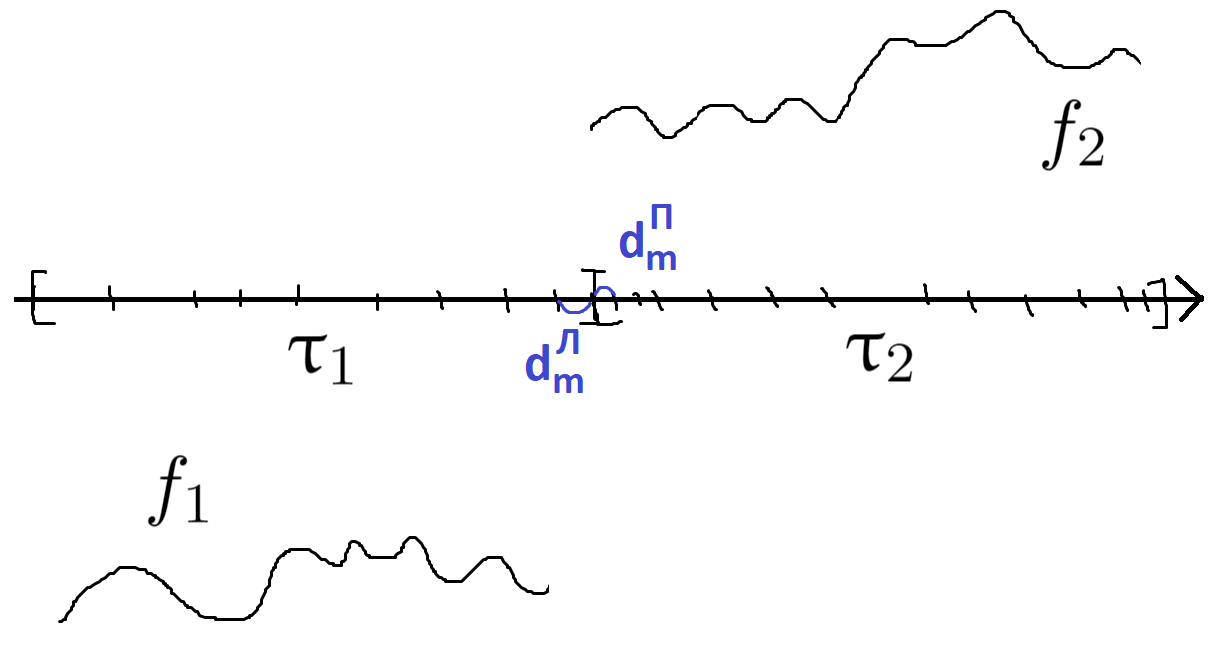
\includegraphics[scale=0.3]{Gap}

    Мог произойти разрыв, но $|f| \leqslant M \Rightarrow \upomega(f,[a,b]) < W$
    $$\sum \upomega(f,d_k)\Delta_k = S^*(f, \uptau)-S_*(f, \uptau) \leqslant S^*(f, \uptau_1)-S_*(f, \uptau_1) + S^*(f, \uptau_2)-S_*(f, \uptau_2) + $$
    $$+d_m^\text{Л} \Delta_m^\text{Л} + d_m^\text{П} \Delta_m^\text{П} \leqslant (d_m=d_m^\text{Л} \cup d_m^\text{П},\ \w{\updelta}=\min(\updelta_1, \updelta_2, \frac{\E}{W})) 2 \E + W \w{\updelta} < 3 \E$$
\end{proof}

\newpage
\section{Свойства интеграла Римана (линейность; аддитивность; свойства, связанные с неравенствами).}

\begin{definition}
    Если $a < b$, то  $\int\limits^a_b f=-\int\limits^b_a f$ и $\int\limits^a_a = 0$
\end{definition}

\begin{Property}[1, линейность]
    \[\forall f,g \in R[a,b], \upalpha, \upbeta \in \R \Rightarrow \int\limits^a_b (\upalpha f + \upbeta g) = \upalpha \int\limits^a_b f + \upbeta \int\limits^a_b g\]
\end{Property}

\begin{proof}
    Знаем, что $\upalpha f + \upbeta g \in R[a,b],$
    $$S(\upalpha f + \upbeta g,  \uptau, \xi) = \upalpha S(f, \uptau, \xi) + \upbeta S(g,  \uptau, \xi) \text{ (очевидно из определения сумм Римана)}$$
\end{proof}

\begin{Property}[2, аддитивность]
    \[\forall f \in R[a,b],\ a<c<b \Rightarrow \int\limits^a_b f = \int\limits^a_c f + \int\limits^c_b f\]
\end{Property}

\begin{proof}
Очевидно (аналогично прошлому)
\end{proof}

\begin{Property}[3]
    \[\forall f \in R[a,b],\ a<b,\ f \geqslant 0 \Rightarrow \int\limits_a^b f \geqslant 0\]
\end{Property}

\begin{proof}
    Очевидно из определения суммы Римана
\end{proof}

\begin{Property}[4]
    \[\forall f,g \in R[a,b],\ g(x) \leqslant f(x)\ \forall x \in [a,b], a<b \Rightarrow \int\limits^a_b g \leqslant \int\limits^a_b f\]
\end{Property}

\begin{proof}
    Очевидно, если взять одно разбиение и оснащение
\end{proof}

\begin{Property}[5]
    \[\forall f \in R[a,b],\ m \leqslant f(x) \leqslant M\ \forall x \in [a,b], a<b \Rightarrow m(b-a) \leqslant \int\limits^a_b f \leqslant M(b-a)\]
\end{Property}

\begin{proof}
    С использованием предыдущего свойства взять интеграл
\end{proof}

\begin{Property}[6]
    \[f \in R[a,b],\ m = \inf\limits_{[a,b]} f,\ M = \sup\limits_{[a,b]} f \Rightarrow \e \upmu \in [m,M]: \int\limits^a_b f =\upmu (b-a)\]
\end{Property}

\begin{Proof}
    \[\upmu=\frac{\int\limits^a_b f}{b-a} \in [m,M] \text{ (по предыдущему неравенству)}\]
\end{Proof}

\begin{Property}[7]
    \[f \in C[a,b], \Rightarrow \e \xi \in [a,b]: \int\limits^a_b f = f(\xi) (b-a)\]
\end{Property}

\begin{proof}
    По теореме о промежуточном значении (Больцано-Коши) используя предыдущее свойство
\end{proof}

\begin{Property}[8]
    \[f \in R[a,b], \Rightarrow |\int\limits^a_b f| \leqslant \int\limits^a_b |f|\]
\end{Property}

\begin{proof}
    $-|f| \leqslant f \leqslant |f| \Rightarrow -\int\limits^a_b |f| \leqslant \int\limits^a_b f \leqslant \int\limits^a_b |f| \Rightarrow |\int\limits^a_b f| \leqslant \int\limits^a_b |f|$
\end{proof}

\newpage
\section{Первая теорема о среднем. Следствие для непрерывных функций.}

\begin{Theorem}
    \[f,g \in R[a,b],\ g \geqslant 0,\ m \leqslant f \leqslant M\] \[\forall x \in [a,b] \Rightarrow \e \upmu \in [m,M]: \int\limits^a_b f g = \upmu \int\limits^a_b g\]
\end{Theorem}

\begin{proof}
    $m g \leqslant f g \leqslant Mg \Rightarrow m \int\limits^a_b g \leqslant \int\limits^a_b f g \leqslant M \int\limits^a_b g$
   	\[\frac{m \int_b^a g}{\int_b^a g} \leq \frac{\int_b^a fg}{ \int_b^a g} \leq \frac{M \int_b^a g}{\int_b^a g}\]
	\[m \leq \frac{\int_b^a fg}{\int_b^a g} \leq M\]
    а) $\int\limits^a_b g = 0$, тогда $\upmu$ - любое.\\
    б) $\int\limits^a_b g \neq 0 \Rightarrow \upmu:=\frac{\int\limits^a_b f g}{\int\limits^a_b g} \in [m,M]$
\end{proof}

\begin{consequence}
    Eсли $f \in C[a,b],\ g \in R[a,b],\ g \geqslant 0 \Rightarrow \e \xi \in [a,b]: \int\limits^a_b f g = f(\xi) \int\limits^a_b g$
\end{consequence}


\begin{proof}
    По теореме о промежуточном значении (Больцано-Коши) используя неравенство из последнего доказательства для $m=\inf\limits_{[a,b]} f,\ M=\sup\limits_{[a,b]} f$
\end{proof}

\newpage
\section{Формула Ньютона-Лейбница. Теорема об интеграле с переменным верхним пределом.}

\begin{definition}
	\[E \subset \R, \q F : E \to \R \q f : E \to \R\]
	\[\text{Тогда } F \text{ называется первообразной f, если } F'(x) = f(x) \q \forall  x \in  E\]
\end{definition}

\begin{utv}
    $F_1, F_2$ - первообразные $f$ на $E$, тогда:
    $$F(x_1)-F(x_2)=\const \text{ (т. Лагранжа)}$$
\end{utv}

\begin{Theorem} [формула Ньютона-Лейбница]
    \[f \in R[a,b],\text{ F -первообразная f, тогда:}\]
    $$\int\limits_a^b f = F(b) - F(a) = F |_a^b$$
\end{Theorem}

\begin{proof}
    $\forall \uptau$ на $[a,b]$ по теореме Лагранжа:
    $$\e \xi_k \in [x_k, x_{x+1}]:\ F(x_{k+1})-F(x_k) = F'(\xi_k)(x_{k+1}-x_k) = f(\xi_k) \Delta_k$$
    \\
    Так как $f \in R[a,b] \Rightarrow \forall \E > 0\ \e \updelta > 0: \forall \uptau: \ \uplambda(\uptau) < \updelta,\ \forall \xi \ |S(f, \uptau, \xi) - I| < \E$
    \\
    Возьмём оснащение $\xi$ из теоремы Лагранжа:
    $$S(f, \uptau, \xi) = \sum\limits_{k=0}^{n-1} f(\xi_k) \Delta_k = \sum\limits_{k=0}^{n-1} (F(x_{k+1})-F(x_k)) = F(b) - F(a)$$
\end{proof}

\begin{definition}
    $E \subset \R$, \q E - невырожденный промежуток,
	\[f : E \to  \R \q \forall \alpha, \beta \in E : \q \alpha < \beta \q f \in R[\alpha, \beta] \q \text{ для }a \in E
	\text{ (фиксированного)}\]
	\[F(x):=\int\limits_a^x f(t) dt \text{ - интеграл с переменным верхним пределом}\]
	\[F : E \to \R\]
\end{definition}

\begin{theorem}
    $f \in R[a,b],\ F(x) = \int\limits_a^x f(t) dt$, тогда:
    \begin{enumerate}
        \item $F \in C[a,b]$
        \item (теорема Барроу) Если $f$ - непр. в т. $x_0 \in [a,b]$, то $F'(x_0)=f(x_0)$
    \end{enumerate}
\end{theorem}

\begin{proof}
    $x \in [a,b],\ h:x+h \in [a,b]$
    \\
    1) $F(x+h)-F(x)= \int\limits_a^{x+h} f - \int\limits_a^x f = \int\limits_a^{x+h} f + \int\limits_x^a f = \int\limits_x^{x+h} f$

    Так как $f \in R[a,b] \Rightarrow \e M \in \R: |f|< M$, значит:
    \[\abs{F(x + h) - F(x)} \leq \abs{\int_x^{x + h} f } \leq \int_x^{x + h}\abs{f} \leq M \abs{h} \]
    Кроме того, $\forall \E > 0,\ \updelta = \frac{\E}{M}$ если $|h| < \updelta \Rightarrow |F(x+h)-F(x)|  < \E$
    \\
2) Рассмотрим $\abs{\frac{F(x_0+h)-F(x_0)}{h}-f(x_0)} =|\frac{1}{h} \int\limits_{x_0}^{x_0+h} f(t) dt - f(x_0) \frac{1}{h} \int\limits_{x_0}^{x_0+h} dt| =$

    $=\frac{1}{|h|} |\int\limits_{x_0}^{x_0+h} (f(t)-f(x_0)) dt| \leqslant \frac{1}{|h|}|\int\limits_{x_0}^{x_0+h} \E dt| = \E$

    (при $|h| < \updelta\ \forall \E > 0\ \e \updelta > 0: |t-x_0|<\updelta \Rightarrow |f(t)-f(x_0)|< \E$)
\end{proof}

\begin{Consequence}
    \[F \in C[a,b] \Rightarrow \e F: F'(x)=f(x)\ \forall x \in [a,b]\]
\end{Consequence}

\begin{example}
    $f(x) = |x|,\ F(x) = \int\limits_0^x |t| dt =
     \begin{cases}
       \dfrac{t^2}{2} \Big|_0^x,& x \geqslant 0\\
       \\
       -\dfrac{t^2}{2} \Big|_0^x,& x < 0
     \end{cases}$
\end{example}

\begin{example}
    $f(x) =
     \begin{cases}
       1,& x \geqslant 0
       \\
       -1,& x < 0
     \end{cases}$

    $F(x) = |x| \ \forall x \neq 0$, видно что неверно для первообразной, но:
    \begin{definition}
        F - "почти первообразная"$,$ если:
        \begin{enumerate}
            \item $F'(x) = f(x)\ \forall x \in [a,b] \setminus \{t_1, ... t_n\}$
            \item $F \in C[a,b]$
        \end{enumerate}
    \end{definition}

    \begin{example}
        Пример для "почти первообразной". Найти $\int\limits_0^2 f(x)$, для $f(x) = \max(1,x)$

        $F(t) \os{?}{=}
         \begin{cases}
           t,& t \in [0,1]
           \\
           \frac{t^2}{2},& t \in [1,2]
         \end{cases}$

        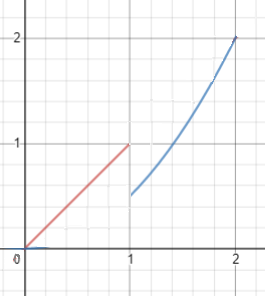
\includegraphics[scale=0.5]{FirstGraph}

        Попробуем использовать Н-Л: $F(t) \big|_0^2 = F(2) - F(0) = 2$ \\Неверно, потому что это не первообразная и даже не "почти первообразная". Поправим F(x):

        $F(t) =
         \begin{cases}
           t,& t \in [0,1]
           \\
           \frac{t^2}{2} + \frac{1}{2},& t \in [1,2]
         \end{cases}$

        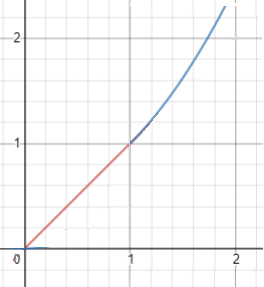
\includegraphics[scale=0.5]{SecondGraph}

        Это уже "почти первообразная"\ можно применять Н-Л.
    \end{example}
\end{example}

\newpage
\section{Формула интегрирования по частям в интеграле Римана. Применение: формула Валлиса.}
\hypertarget{12q}{}
\begin{Theorem}
    \[\text{$F,G$ - первообразные $f,g \in R[a,b]$ на $[a,b]$, тогда } \int\limits_a^b F g = F G |_a^b-\int\limits_a^b f G\]
    $$(\int\limits_a^b u v' = u v |_a^b - \int\limits_a^b u' v)$$
\end{Theorem}

\begin{Proof}
    \[(F G)' = f G + F g, \text{ по ф-ле Н-Л: }\int\limits_a^b (F G)' = F G |_a^b = \int\limits_a^b f G + |_a^b F g\]
\end{Proof}

\begin{example}
    Если $I_m := \int\limits_0^{\frac{\pi}{2}} \sin^m x dx = \int\limits_0^{\frac{\pi}{2}} \cos^m x dx$, то:

    \[
    I_m =
     \begin{cases}
       \dfrac{\pi}{2} \dfrac{(m-1)!!}{m!!}, &\text{$m$ - четное}\\ \\
       \dfrac{(m-1)!!}{m!!}, &\text{$m$ - нечетное}
     \end{cases}
    \]
\end{example}

\begin{Proof}
    \begin{multline*}
        $$I_m = \int\limits_0^{\frac{\pi}{2}} \sin^m x dx = \int\limits_0^{\frac{\pi}{2}} (-\cos x)' \sin^{m-1} x dx =\\= - \cos x \sin^{m-1} x |_0^{\frac{\pi}{2}} - \int\limits_0^{\frac{\pi}{2}} \cos^2 x (m-1) \sin^{m-2} x dx =\\= (m-1) \int\limits_0^{\frac{\pi}{2}} (\sin^{m-2} x - \sin^m x) dx = (m-1)(I_{m-2}-I_m)$$
    \end{multline*}

    \[I_m=\frac{m-1}{m} I_{m-2},\ I_0=\frac{\pi}{2},\ I_1= 1,\ I_2=\frac{\pi}{2} \frac{1}{2},\ I_{2k}=\frac{\pi}{2} \frac{1}{2} \frac{3}{4} ... \frac{2k-1}{2k} = \frac{\pi}{2} \frac{(2k-1)!!}{(2k)!!}\]
\end{Proof}

\begin{Theorem}[Формула Валлиса]
    \[\lim\limits_{n \rightarrow \infty} \frac{2*2*4*4*...*(2n)(2n)}{1*3*3*5*5...(2n-1)(2n+1)} = \dfrac{\pi}{2}$ (или $\lim\limits_{n \rightarrow \infty} \frac{1}{n} (\frac{(2n)!!}{(2n-1)!!})^2 = \pi)\]
\end{Theorem}

\begin{proof}
    $\forall x \in [0, \frac{\pi}{2}]$ верно $\int\limits_0^{\frac{\pi}{2}} \sin^{2n+1} x \leqslant \int\limits_0^{\frac{\pi}{2}} \sin^{2n} x \leqslant \int\limits_0^{\frac{\pi}{2}} \sin^{2n-1} x$
    $$\frac{(2n)!!}{(2n+1)!!} \leqslant \frac{\pi}{2} \frac{(2n-1)!!}{(2n)!!} \leqslant \frac{(2n-2)!!}{(2n-1)!!}$$
    $$A_n=\frac{((2n)!!)^2}{(2n-1)!!(2n+1)!!} \leqslant \frac{\pi}{2} \leqslant \frac{(2n)!! (2n-2)!!}{((2n-1)!!)^2}=B_n$$
    \begin{multline*}
        $$B_n - A_n = \frac{(2n)!! (2n-2)!!}{((2n-1)!!)^2} - \frac{((2n)!!)^2}{(2n-1)!!(2n+1)!!} =\\= (\frac{(2n)!!}{(2n-1)!!})^2 (\frac{1}{2n} - \frac{1}{2n+1})=(\frac{((2n)!!)^2}{(2n-1)!!(2n-1)!!})\frac{1}{(2n+1)(2n)}=\\
        =A_n \frac{1}{2n} \leqslant \frac{\pi}{2} \frac{1}{2n} \rightarrow\limits_{n \rightarrow \infty} 0 \Rightarrow \lim\limits_{n \rightarrow \infty} A_n = \lim\limits_{n \rightarrow \infty} B_n=\frac{\pi}{2}$$
    \end{multline*}
\end{proof}

\newpage
\section{Формула Тейлора с остаточным членом в интегральной форме.}

\begin{Theorem}
    \begin{multline*}
        $$f \in C^{n+1} ([a,b]) \Rightarrow f(b)=\sum\limits_{k=0}^n \frac{f^{(k)}(a)}{k!} (b-a)^k + R_n (b,a), \\ \text{ где }R_n(b,a)=\frac{1}{n!} \int\limits_a^b f^{(n+1)}(t) (b-t)^n dt$$
    \end{multline*}
\end{Theorem}

\begin{Remark}
    \[f \in C^{n+1}([a,b]) \Rightarrow f^{(n+1)} \in C[a,b] \Rightarrow \e \xi \in [a,b]:\]
    \[R_n=\frac{1}{n!} f^{(n+1)} (\xi) \int\limits_a^b(b-t)^n dt = \frac{-f^{(n+1)}(\xi)}{n!} \frac{(b-t)^{n+1}}{n+1} \Big|_a^b = \frac{-f^{(n+1)}(\xi)}{(n+1)!} (b-a)^{n+1}\]
\end{Remark}

\begin{proof}[по индукции]
    1) $n=0$

    $f(b)=f(a)+\int\limits_a^b f'(t) dt$ - формула Н-Л
    \\
    2) Инд. переход. Пусть для $n-1$ - доказано, $f \in C^{n-1}[a,b] \subset C^n [a,b]$, по инд. предположению:
    $$f(b)=\sum\limits_{k=0}^{n-1} \frac{f^{(k)}(a)}{k!} (b-a)^k + R_{n-1} (*)$$
    $$R_{n-1} = \frac{1}{(n-1)!} \int\limits_a^b f^{(n)}(t) (b-t)^{n-1} dt =
    \begin{bmatrix}
    u=f^{(n)}(t)\\
    dv=(b-t)^{n-1} dt
    \end{bmatrix} = $$
    $$= \frac{1}{(n-1)!} (-f^{(n)}(t)\frac{(b-t)^n}{n}\bigg|_a^b + \int\limits_a^b f^{(n+1)}(t)\frac{(b-t)^n}{n} dt) = $$
    $$=\frac{1}{(n)!} (f^{(n)}(a)(b-a)^n+ \int\limits_a^b f^{(n+1)}(t)(b-t)^n dt)\text{ - подставить в $(*)$}$$
\end{proof}

\newpage
\section{Формула интегрирования по частям в интеграле Римана. Вторая теорема о среднем.}

Формулу интегрирования по частям см. в  \hyperlink{12q}{12 билете.}
\begin{Theorem}[Бонне или вторая теорема о среднем]
    \begin{multline*}
        $$f \in C[a,b],\ g\in C^1[a,b], g - \text{монотонна} \\
        \Rightarrow \e \xi \in [a,b]: \int\limits_a^b f g = g(a) \int\limits_a^\xi f  + g(b) \int\limits_\xi^b f$$
    \end{multline*}
\end{Theorem}

\begin{proof}
    (для $g\nearrow$) $F(x):=\int\limits_a^x f \Rightarrow F'=f$
    $$\int\limits_a^b f g = \int\limits_a^b F' g = F g |_a^b - \int\limits_a^b F g' = F(b)g(b) - F(a)g(a) - \int\limits_a^b F g' = $$
    $$\text{(т.к. $g\nearrow$ $g \geqslant 0 \Rightarrow$ по т. о среднем $\e \xi \in [a,b]:)$}$$
    $$= F(b) g(b) -  g(a) F(a) - F(\xi)\int\limits_a^b g' = g(b)(F(b)-F(\xi))+g(a)(F(\xi)-F(a))$$
\end{proof}

\newpage
\section{Замена переменной в определенном интеграле (две формулировки, доказательство одной).}


\begin{Theorem}
    \[\upvarphi \subset C^1 [\upalpha,\upbeta],\ f \in C(\upvarphi([\upalpha,\upbeta])),\text{ тогда } \int\limits_{\upvarphi(\upalpha)}^{\upvarphi(\upbeta)} f = \int\limits_{\upalpha}^{\upbeta} (f \circ \upvarphi) \upvarphi'\]
\end{Theorem}

\begin{proof}
    $f \in C(\upvarphi([\upalpha,\upbeta])) \Rightarrow \e F: F'=f$
    $$(F \circ \upvarphi)' = (F' \circ \upvarphi) \upvarphi' = (f \circ \upvarphi) \upvarphi' \Rightarrow \int\limits_\upalpha^\upbeta (f \circ \upvarphi) \upvarphi' =( F \circ \upvarphi) (\upbeta) - (F \circ \upvarphi) (\upalpha)$$
    $$ \int\limits_{\upvarphi(\upalpha)}^{\upvarphi(\upbeta)} f = F(\upvarphi(\upbeta)) - F(\upvarphi(\upalpha)) = \int\limits_\upalpha^\upbeta (f \circ \upvarphi) \upvarphi'$$
\end{proof}

\begin{Theorem}
    \begin{multline*}
        $$f \in R[a,b],\ \upvarphi \in C^1 [\upalpha, \upbeta],\ \upvarphi \text{ - строго возрастает}, \\
        \upvarphi(\upalpha) = a,\q \upvarphi(\upbeta) = b,
        \text{ тогда } \int\limits_a^b f = \int\limits_\upalpha^\upbeta (f \circ \upvarphi) \upvarphi'$$
    \end{multline*}
\end{Theorem}

\begin{Example}
    \[\int\limits_0^1 \sqrt{1-x^2} dx,\q \upvarphi(t) = \cos t,\q \upvarphi(\upalpha)=0$, $\upvarphi(\upbeta)=1\]

    \[\int\limits_0^1 \sqrt{1-x^2} dx = - \int\limits_{\frac{\pi}{2}}^0 \sqrt{1-\cos^2 t} \sin t dt = - \int\limits_{\frac{\pi}{2}}^0 \frac{1 - \cos 2t}{2} dt = (-\frac{t}{2} + \frac{\sin 2t}{4}) \Big|_{\frac{\pi}{2}}^0 = \frac{\pi}{4}\]
\end{Example}

\newpage
\begin{Reminder} [про ряды]\
\begin{definition}
    Числовой ряд из элементов $\{a_j\}_{j \in \N}$ - это $\sum\limits_{j=1}^\infty a_j$
\end{definition}

\begin{definition}
    Частичная сумма ряда $S_n = \sum\limits_{j=1}^n a_j$
\end{definition}

\begin{definition}
    Говорят, что сумма ряда $S=\sum\limits_{j=1}^\infty a_j=\lim\limits_{n \rightarrow \infty} S_n$
\end{definition}

\begin{Remark}
    \[\text{Ряд $\sum\limits_{j=1}^\infty a_j$ сходится или расходится одновременно с рядом $\sum\limits_{j=N}^\infty a_j$}\]
\end{Remark}

\begin{Theorem} [необходимое условие сходимости]
    \[\text{Если $\sum\limits_{j=1}^\infty a_j$ - cходится, то $\lim\limits_{j \rightarrow \infty} a_j = 0$}\]
\end{Theorem}

\begin{definition}
    Ряд Лейбница $\sum\limits_{j=0}^\infty (-1)^j a_j$, $a_j>0$, где $\lim\limits_{j \rightarrow \infty} a_j =0$, $a_j \searrow$
\end{definition}

\begin{theorem}\ \\
    Пусть $\sum\limits_{j=0}^\infty (-1)^j a_j$ - ряд Лейбница, тогда:
    \begin{enumerate}
        \item Ряд Лейбница сходится
        \item $S_{2n} \searrow$, $S_{2n-1} \nearrow$
        \item $|S-S_n|<a_{n+1}$
    \end{enumerate}
\end{theorem}

\begin{theorem}\ \\
    Критерий Коши для числовых последовательностей.

    $\sum\limits_{j=1}^\infty a_j$ - сх $\lra \forall \E > 0\ \e N: \forall m>n>N\ |S_m-S_n|<\E$
\end{theorem}
\end{Reminder}

\newpage
\section{Признаки сравнения для положительных рядов.}

\begin{definition}
    Если $a_j \geqslant 0$, то $\sum\limits_{j=1}^\infty a_j$ - положительный ряд
\end{definition}

\begin{theorem}\ \\
    Положительный ряд сходится $\lra S_n$ - ограничены
\end{theorem}

\begin{consequence} \ \\
    Пусть $0 \leqslant a_j \leqslant b_j$, тогда:
    \begin{enumerate}
        \item $\sum b_j$ - сх $\Rightarrow$ $\sum a_j$ - сх (первый признак сходимости)
        \item $\sum a_j$ - расх $\Rightarrow$ $\sum b_j$ - расх (первый признак сравнения)
    \end{enumerate}
\end{consequence}

\begin{Consequence}
    \[a_k \geqslant 0,\ b_k \geqslant 0,\ \e c,d > 0\ \e N: \forall n > N\ 0 < c \leqslant \frac{a_n}{b_n} \leqslant d \leqslant \infty\]
    Тогда $\sum a_k$ и $\sum b_k$ сх. или расх. одновременно
\end{Consequence}

\begin{proof}
    (т.е. $\sum a_k$ - сх $\lra$ $\sum b_k$ - сх)

    ($\Leftarrow$) $0 \leqslant a_n \leqslant d b_n$ т.к. $d b_n$ - сх $\Rightarrow$ $a_n$ - сх

    ($\Rightarrow$) $0 \leqslant c b_n \leqslant a_n$ т.к. $a_n$ - сх $\Rightarrow$ $c b_n$ - сх $\Rightarrow$ $b_n$ - сх
\end{proof}

\begin{consequence} [второй признак сравнения]
    Пусть $a_n, b_n \geqslant 0$, тогда если

    $\e \lim\limits_{n \rightarrow \infty} \dfrac{a_n}{b_n} = L \in (0, + \infty)$, то $\sum a_n$ и $\sum b_n$ сх или расх одновременно
\end{consequence}

\begin{proof}
    Возьмём $\E:=\dfrac{L}{2} \Rightarrow \e N: \forall n > N$ $\big|\dfrac{a_n}{b_n} - L\big| < \dfrac{L}{2} \Rightarrow$

    $0 < \dfrac{L}{2} < \dfrac{a_n}{b_n} < \dfrac{3L}{2} < +\infty \Rightarrow$ по предыдущему следствию верно
\end{proof}

\newpage
\section{Признаки Даламбера и Коши для положительных рядов.}

\begin{theorem} [радикальный признак Коши для положительных рядов]
    $a_k \geqslant 0$, $c:=\overline{\lim\limits_{k \rightarrow \infty}} \sqrt[k]{a_k}$

    Если $c < 1$, то $\sum a_k$ - сх

    Если $c > 1$, то $\sum a_k$ - расх
\end{theorem}

\begin{proof}

    а) $0 \leqslant c < 1$
    \begin{figure}[H]
        \centering
        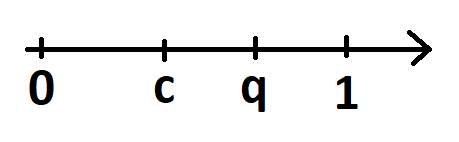
\includegraphics[width=3cm]{pics/Cauchy1}
    \end{figure}
    $q := \frac{c+1}{2}$, $c<q<1$, по характеристике $\overline{\lim}: \e N: \forall n > N\ \sqrt[n]{a_n} < q$

    т.к. $0 \leqslant a_n < q^n$ и $\sum q^n$ - сх $\Rightarrow \sum a_n$ - сх
    \\
    б) $c > 1$
    \begin{figure}[H]
        \centering
        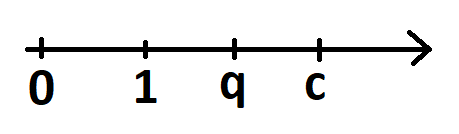
\includegraphics[width=3cm]{pics/Cauchy2}
    \end{figure}
    $q := \frac{c+1}{2}$, $1<q<c$, по характеристике $\overline{\lim}:$ $\forall N: \e n > N$ $\sqrt[n]{a_n} > q$

    т.е. $\e$ бесконечное мн-во $\sqrt[n_k]{a_{n_k}} > q$, $a_{n_k} > q^{n_k} > 1$

    $\Rightarrow \lim a_{n_k} \neq 0 \Rightarrow \sum a_n$ - расх
\end{proof}

\begin{theorem} [признак Даламбера сходимости положительных рядов]
    $a_k \geqslant 0$, $\mathcal{D}:=\lim\limits_{k \rightarrow \infty} \frac{a_{k+1}}{a_k}$

    Если $\mathcal{D} < 1$, то $\sum a_k$ - сх

    Если $\mathcal{D} > 1$, то $\sum a_k$ - расх
\end{theorem}

\begin{proof}
    а) $\mathcal{D} < 1$, $q := \frac{\mathcal{D} + 1}{2}$ $\E := \frac{1 - \mathcal{D}}{2}$
    \begin{figure}[H]
        \centering
        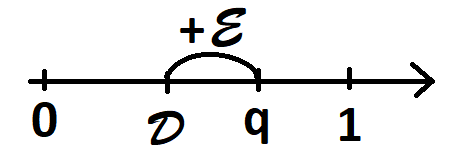
\includegraphics[width=3cm]{pics/D'Alembert1}
    \end{figure}
    $\e N: \forall k>N$ $\mathcal{D}-\E < \frac{a_{k+1}}{a_k} < \mathcal{D}+\E = q$ - геом пр. $q < 1$

    $a_{k+1} < q a_k < q^2 a_{k-1} < ... < q^{k-N+1} a_N$, $\sum q^{k-N+1} a_k$ - сх $\Rightarrow \sum a_{k+1}$ - сх по первому пр. сходимости
    \\
    б) $\mathcal{D} < 1$, $q := \frac{\mathcal{D} + 1}{2}$ $\E := \frac{\mathcal{D} - 1}{2}$
    \begin{figure}[H]
        \centering
        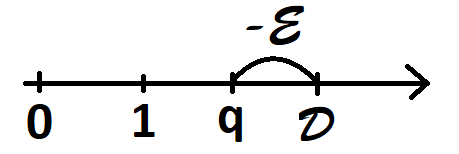
\includegraphics[width=3cm]{pics/D'Alembert2}
    \end{figure}
    $\e N: \forall k>N$ $q = \mathcal{D}-\E < \frac{a_{k+1}}{a_k} < \mathcal{D}+\E$, $q > 1$

    $a_{k+1}> q a_k > q^2 a_{k-1} > ... >q^{k-N+1} a_N$, $\sum q^{k-N+1} a_N$ - расх $\Rightarrow \sum a_{k+1}$ - расх по первому пр. сравнения
\end{proof}

\newpage
\section{Абсолютная и условная сходимость рядов. Сходимость следует из абсолютной сходимости.}
\hypertarget{q18}{}

\begin{definition}
    $\sum\limits_{j=1}^\infty a_j$ - сх абсолютно, если $\sum\limits_{j=1}^\infty |a_j|$ - сх
\end{definition}

\begin{definition}
    Ряд сходится условно если сходится, но не абсолютно
\end{definition}

\begin{theorem}
    Если ряд сходится абсолютно, то он сходится
\end{theorem}

\begin{proof} \ \\
    $\sum\limits_{j=1}^\infty |a_j|$ - сх, по критерию Коши $\forall \E > 0\ \e N: \forall m>n>N:$

    $$||a_{n+1}|+...+|a_m||<\E \text{, по неравенству треугольника:}$$
    $$|a_{n+1}+...+a_m|<\E \Rightarrow \sum\limits_{j=1}^\infty a_j \text{ - сх.}$$
\end{proof}

\newpage
\section{Абсолютная и условная сходимость. Пример: $\sum\limits_{n=1}^\infty \frac{(-1)^{n-1}}{n}$}

Определения см. в \hyperlink{q18}{предыдущем} билете. \\
Ряд не сходится абсолютно, т.к. $\sum\limits_{n=1}^\infty \big|\frac{(-1)^{n-1}}{n}\big|=\sum\limits_{n=1}^\infty \frac{1}{n}$ - расх. ряд, т.к.:

\begin{theorem} [критерий Коши сходимости последовательности]
    $x_n$ - сх $\lra x_n$ - сх в себе.
\end{theorem}
Покажем, что для $S_n=1+\frac{1}{2}+...+\frac{1}{n}$ $\e \E > 0: \forall N\ \e m,n \geqslant N: |x_m-x_n|>\E$:
$$\text{Возьмём }\E = \frac{1}{4}\text{ n }=N,\ m=2N:$$
$$|S_{2N} - S_N| = \Big|\frac{1}{N+1}+...+\frac{1}{2N}\Big| > N \frac{1}{2N} = \frac{1}{2} > \E$$ \\
Но ряд сходится (значит условно сходится) по признаку Лейбница (или это можно показать прямо, доказав что $S_{2n} \nearrow$ и ограничена сверху единицей, а $S_{2n+1}=S_{2n}$ в пределе)

\newpage
\section{Перестановка абсолютно сходящегося ряда. Теорема Римана (б/д).}

\begin{definition}
    Пусть есть ряд $\sum\limits_{k=1}^\infty a_k$ и биективная функция $\upvarphi: \N \rightarrow \N$, тогда ряд $\sum\limits_{k=1}^\infty a_{\upvarphi(k)}$ называется перестановкой ряда $\sum\limits_{k=1}^\infty a_k$
\end{definition}

\begin{theorem} [Римана v1] \ \\
    Пусть ряд $\sum a_n$ - условно сходится, тогда:
    \[\forall S \in \overline{\R}\ \e \upvarphi: \N \rightarrow \N: \sum a_{\upvarphi(k)} = S\]
\end{theorem}

\begin{definition}
    $a_k^+ = \max\{a_k, 0\}$, $a_k^- = \max\{-a_k, 0\}$
\end{definition}

\begin{theorem} [Дирихле, о перестановке абсолютно сходящегося ряда] \ \\
    Если $\sum\limits_{n=1}^\infty a_n= S$ сх абсолютно, то

    $\forall \upvarphi: \N \rightarrow \N$, где $\upvarphi$ - биекция $\Rightarrow \sum\limits_{n=1}^\infty a_{\upvarphi(n)} = S$
\end{theorem}

\begin{proof}\\
    а) Пусть $a_n \geqslant 0\ \forall n \in \N$

    $S := \sum\limits_{n=1}^\infty a_n$ - сх $\lra$ все частичные суммы ограничены,  $S_n \leqslant S\ \forall n \in \N$

    Частичные суммы $\sum\limits_{k=1}^n a_{\upvarphi(k)}$ обозначим перестановками ряда $T_n := \sum\limits_{k=1}^n a_{\upvarphi(k)}$

    Пусть $m:=\max \{\upvarphi(1), \upvarphi(2), ..., \upvarphi(n) \}$

    $T_n \leqslant S_m := \sum\limits_{n=1}^m a_{\upvarphi(a_n)} \leqslant S \Rightarrow T_n \nearrow$ - огр $\lra$ ряд $T := \sum\limits_{n=1}^\infty a_{\upvarphi(a_n)}$ сходится.

    Предельный переход даёт $T \leqslant S$, но так как $S$ - тоже перестаовка $T$ $\Rightarrow$ $S \leqslant T$

    Значит $S=T$, то есть $\sum\limits_{n=1}^\infty a_n = \sum\limits_{n=1}^\infty a_{\upvarphi(a_n)}$
    \\
    б) Общий случай, $a_k \in \R $

    $a_k = a_k^+ - a_k^-$, $|a_k| = a_k^+ + a_k^- \Rightarrow a_k^+ = \frac{a_k + |a_k|}{2},\ a_k^-=\frac{|a_k|-a_k}{2}$

    т.к. $\sum a_k$ - сх абсолютно $\Rightarrow \sum |a_k|$ - сх

    $\Rightarrow \sum a_k^+,\ \sum a_k^-$ - сх (причем абсолютно)

    $$\sum\limits_{k=0}^\infty a_{\upvarphi(k)} = \sum\limits_{k=0}^\infty (a_{\upvarphi(k)}^+ - a_{\upvarphi(k)}^-) = \sum\limits_{k=0}^\infty a_{\upvarphi(k)}^+ - \sum\limits_{k=0}^\infty a_{\upvarphi(k)}^- =\text{ (п. а) }\sum\limits_{k=0}^\infty (a_k^+ - a_k^-) = \sum\limits_{k=0}^\infty a_k$$
\end{proof}

\begin{theorem} [Римана v2]
    Пусть ряд $\sum a_n$ - условно сходится. Тогда $\sum a_n^+ - \sum a_n^- = + \infty$
\end{theorem}

\begin{proof}
    Можно доказать одну из теорем
\end{proof}

\newpage
\section{Асимптотика частичных сумм расходящегося ряда (случай гармонического ряда). Постоянная Эйлера.}

\[\frac{1}{1+k} = \frac{\frac{1}{k}}{\frac{1}{k}+1} < \ln(1+\frac{1}{k}) < \frac{1}{k} \Rightarrow 0 < \frac{1}{k} - \ln(1+\frac{1}{k})< \frac{1}{k}-\frac{1}{k+1}\]

Значит, \begin{multline*}
    $$0 < \sum\limits_{k=1}^n \big(\dfrac{1}{k} - \ln(1+\dfrac{1}{k})\big) < \sum\limits_{k=1}^n \big(\dfrac{1}{k} - \dfrac{1}{k+1}\big) = \\
    =1 - \cancel{\frac{1}{2}} + \cancel{\frac{1}{2}} - \cancel{\frac{1}{3}} + \cancel{\frac{1}{3}} -...+ \cancel{\frac{1}{n}} - \frac{1}{n-1} =\\
    =1 - \frac{1}{n+1} = \frac{n}{n+1} < 1\ \forall n \in \N$$
\end{multline*}
\\
$\Rightarrow S_n := \sum\limits_{k=1}^n \big(\dfrac{1}{k} - \ln(1+\dfrac{1}{k})\big) \nearrow$ и ограничено сверху $\Rightarrow \e \lim\limits_{n \rightarrow \infty} S_n$

$$\sum\limits_{k=1}^n \ln (1+ \frac{1}{k}) = \sum\limits_{k=1}^n (\ln(k+1) - \ln(k)) = -\ln1+\cancel{\ln2}-\cancel{\ln2}+\cancel{\ln3}-...-\cancel{\ln (n)}+ \ln (n+1) =$$
$$ =\ln (n+1) \Rightarrow \e \lim\limits_{n \rightarrow \infty} \sum\limits_{k=1}^n \frac{1}{k} - \ln (n+1) = \lim\limits_{n \rightarrow \infty} (\sum\limits_{k=1}^n \frac{1}{k} - \ln n)$$

\begin{definition}
    $\upgamma := \lim\limits_{n \rightarrow \infty} (\sum\limits_{k=1}^n \dfrac{1}{k} - \ln n) = 0,5722...$ - постоянная Эйлера
\end{definition}

\newpage
\section{Несобственные интегралы. Примеры. Несобственный интеграл в смысле главного значения. Критерий Больцано-Коши для несобственных интегралов.}

\begin{definition}[1]
    $f: [a, +\infty) \rightarrow \R$, $f \in R[a,b]$ $\forall b \in (a, +\infty).$
    \begin{multline*}
        $$\text{Если }\e \lim\limits_{b \rightarrow \infty} \int\limits_a^b f, \text{ то говорят, что несобственный интеграл} \\
        \int\limits_a^{+\infty} f \text{ - сходится и равен } \lim\limits_{b \rightarrow \infty} \int\limits_a^b f$$
    \end{multline*}
\end{definition}

\begin{definition}[2]
    $f: [a, \upomega) \rightarrow \R$, $-\infty < a < \upomega \leqslant +\infty$ ,\ $f \in R[a,b]$ $\forall b \in (a, +\infty)$.
    \begin{multline*}
        $$\text{Если }\e \lim\limits_{b \rightarrow \upomega_-} \int\limits_a^b f,\text{ то говорят, что несобственный интеграл } \\
        \int\limits_a^{\upomega} f\text{ - сх и равен } \lim\limits_{b \rightarrow \upomega_-} \int\limits_a^b f$$
    \end{multline*}
\end{definition}

\begin{definition}[3]
    $f: \R \rightarrow \R$ и $\forall a<b\in \R: f \in R[a,b]$, тогда $\int\limits_{-\infty}^{+\infty} f := \lim\limits_{a \rightarrow -\infty} \int\limits_a^0 f + \lim\limits_{b \rightarrow +\infty} \int\limits_0^b f$,

    Если оба предела $\e$ и конечны, то говорят что $\int\limits_{-\infty}^{+\infty} f$ - сходится
\end{definition}

\begin{definition}[4]
    Аналогично $\int\limits_{\upomega_1}^{\upomega_2}$, если $f \in R[a,b]$ $\forall[a,b] \subset (\upomega_1,\upomega_2)$. $\int\limits_{\upomega_1}^{\upomega_2} f= \int\limits_{\upomega_1}^c f + \int\limits_c^{\upomega_2}$
\end{definition}

\begin{example}
    \begin{enumerate}
        \item $\upalpha = 1$, $\int\limits_1^{+\infty} \dfrac{dx}{x^\upalpha} = \lim\limits_{b \rightarrow +\infty} \ln |x| \big|_1^b = +\infty$ - расх
        \item $\upalpha > 1$, $\int\limits_1^{+\infty} \dfrac{dx}{x^\upalpha} = \lim\limits_{b \rightarrow +\infty} \dfrac{x^{1-\upalpha}}{1-\upalpha} \Big|_1^b = 0-\dfrac{1}{1-\upalpha}$ - сх
        \item $\upalpha < 1$, $\int\limits_1^{+\infty} \dfrac{dx}{x^\upalpha} =  +\infty$ - расх
    \end{enumerate}
\end{example}

\begin{Example}
    \[\int\limits_{-1}^1 \frac{dx}{x} = \lim\limits_{a \rightarrow 0_-} \int\limits_{-1}^a \frac{dx}{x} + \lim\limits_{b \rightarrow 0_+} \int\limits_{b}^1 \frac{dx}{x}\text{ - расх по опр, т.к. оба предела расх}\]
\end{Example}

\begin{definition}
    $f: \R \rightarrow \R$ и $\forall a<b\in \R: f \in R[a,b]$, тогда (V.P.) $\int\limits_{-\infty}^{+\infty} f := \lim\limits_{A \rightarrow +\infty} \int\limits_{-A}^A f$
\end{definition}

\begin{Example}
    \[(V.P.)\q \int\limits_{-\infty}^{+\infty} x = \lim\limits_{A \rightarrow +\infty} \int_{-A}^A x = \lim\limits_{A \rightarrow +\infty} \frac{x^2}{2} \Big|_{-A}^A = 0\]

    \[(\text{Но }\int\limits_{-\infty}^{+\infty} x = \lim\limits_{a \rightarrow -\infty} \int_a^0 x + \lim\limits_{b \rightarrow +\infty} \int_0^b x\text{ - расх})\]
\end{Example}

\begin{Theorem} [критерий Больцано-Коши для несобственных интегралов]
    \[f: [a, \upomega) \rightarrow \R,\q -\infty < a < \upomega \leqslant +\infty,\q f \in R[a,b]\q \forall b \in (a, +\infty),\text{ тогда:}\]
    \[\int\limits_a^\upomega f\text{ - сх }\lra \q \forall \E > 0\ \e B \in (a, \upomega): \forall b_1,b_2 \in (B, \upomega)\ |\int\limits_{b_1}^{b_2}| < \E\]
\end{Theorem}

\begin{Proof}
    \[\int\limits_a^\upomega f$ - сх $\lra$ $\e \lim\limits_{b \rightarrow \upomega} \int\limits_a^b f \lra \text{(кр Коши для пределов ф.)}\]
    \[\forall \E > 0\ \e \updelta > 0: \forall b_1,b_2 \in (\upomega - \updelta, \upomega)\ |\int\limits_a^{b_1} f - \int\limits_a^{b_2} f| < \E \Rightarrow |\int\limits_{b_1}^{b_2} f| < \E\]
\end{Proof}

\newpage
\section{Свойства несобственных интегралов (линейность, аддитивность, монотонность, формула Ньютона-Лейбница).}

\begin{Property} [1, линейность]
    \[\int\limits_a^\upomega f_1, \int\limits_a^\upomega f_2 \text{ - сх }\Rightarrow \forall k_1, k_2 \in \R \q \int\limits_a^\upomega (k_1 f_1 + k_2 f_2) = k_1 \int\limits_a^\upomega f_1 + k_2 \int\limits_a^\upomega f_2\]
\end{Property}

\begin{Property} [2, монотонность]
    \begin{multline*}
        $$f,g: [a, \upomega) \rightarrow \R,\q f,g \in R[a,b],\q \forall b \subset [a,\upomega),\q f(x) \leqslant g(x), \\ \forall x \in [a, \upomega) \Rightarrow \int\limits_a^\upomega f \leqslant \int\limits_a^\upomega g$$
    \end{multline*}
\end{Property}

\begin{Lemma}
    \begin{multline*}
        $$f:[a, \upomega) \rightarrow \R,\q f \in R[a,b],\ \forall b \in (a, \upomega).\\
        \text{Пусть }c \in (a, \upomega), \text{ тогда } \int\limits_a^\upomega f\text{ и }\int\limits_c^\upomega f \text{ - сх или расх одновременно}$$
    \end{multline*}
\end{Lemma}

\begin{Proof}
    \[\int\limits_a^\upomega f$ - сх $\lra$ $\lim\limits_{b \rightarrow \upomega_-} \int\limits_a^b f = A \in \R\]
    \[\text{Тогда }\int\limits_c^\upomega f=\lim\limits_{b \rightarrow \upomega_-} \int\limits_c^b f = \lim\limits_{b \rightarrow \upomega_-} (\int\limits_a^b f - \int\limits_a^c f) = A - \int\limits_a^c f \in \R \Rightarrow \int\limits_c^\upomega f \text{ - сх}\]
\end{Proof}

\begin{Property} [3, аддитивность]
    \[f: [a, \upomega) \rightarrow \R,\q f \in R[a,b]\ \forall b \subset [a,\upomega)\]

    \[\forall c \in [a, \upomega) \Rightarrow \int\limits_a^\upomega f = \int\limits_a^c f + \int\limits_c^\upomega f, \text{ причем } \int\limits_a^\upomega f \text{ и } \int\limits_c^\upomega f \text{ - сх или расх одновременно}\]
\end{Property}

\begin{property} [4, формула Н-Л] \ \\
    Если $F$ - первообразная $f$, то:
    \[\int\limits_a^\upomega f = \lim\limits_{b \rightarrow \upomega_-} (F(b) - F(a)) =: F \big|_a^{\upomega_-} = F(\upomega_-)-F(a)\]
\end{property}

\begin{Property} [5]
    \[\text{Если }f \in R[a,\upomega]\ (\upomega \in \R),\text{ то (несоб. инт)}\int\limits_a^\upomega f = \int\limits_a^\upomega f \text{(инт Римана)}\]
\end{Property}

\begin{proof}
    $f \in R[a,\upomega] \Rightarrow F(x) := \int\limits_a^x f \in C[a, \upomega]$,
    \\
    (несоб. инт) $\int\limits_a^\upomega f = \lim\limits_{b \rightarrow \upomega} \int\limits_a^b f (=F(b) \text{ (непр. в т $\upomega)$}) = F(\upomega) = \int\limits_a^\upomega f$ (инт Римана)
\end{proof}

\newpage
\section{Свойства несобственных интегралов (интегрирование по частям, замена переменной).}

\begin{Property} [интегрирование по частям]
    \begin{multline*}
        $$\text{Пусть } f,g \in C^1 [a, \upomega),\q \e \lim\limits_{x \rightarrow \upomega_-} f(x) g(x) \in \R, \text{ тогда:}\\
        \int\limits_a^\upomega f' g\text{ и } \int\limits_a^\upomega f g'\text{ - сх или расх одновременно, причем }\\
        \int\limits_a^\upomega f g' = f g |_a^\upomega - \int\limits_a^\upomega f' g (f g |_a^\upomega =  \lim\limits_{x \rightarrow \upomega_-} (f(x) g(x) - f(a) g(a))$$
    \end{multline*}
\end{Property}

\begin{Property} [замена переменной]
    \begin{multline*}
        $$\text{Если }\int\limits_a^\upomega f \text{ - сх},\q \upvarphi: [\upalpha, \upupsilon) \rightarrow [a, \upomega),\q \upvarphi \in C^1 [\upalpha, \upupsilon),\q \upvarphi\text{ - монот.},\\
        \upvarphi(\upalpha)=a,\q \lim\limits_{t \rightarrow \upupsilon} \upvarphi(t) = \upomega,\text{ тогда }\int\limits_a^\upomega f = \int\limits_\upalpha^\upupsilon (f \circ \upvarphi) \upvarphi'$$
    \end{multline*}
\end{Property}

\newpage
\section{Интегральный признак Коши сходимости несобственных интегралов и рядов.}

\begin{theorem}
    Пусть $f: [1, +\infty) \rightarrow [0, +\infty)$, $f \in R[1,A]\ \forall A > 1$, $f$ - строго убывает (можно строго возрастает)
    \\
    Тогда $\int\limits_1^\infty f$ и $\sum\limits_{n=1}^\infty f(n)$ - сх или расх одновременно, причем

    $\sum\limits_{n=1}^\infty f(n+1) \leqslant \int\limits_1^\infty f \leqslant \sum\limits_{n=1}^{\infty} f(n)$
    \begin{figure}[H]
        \centering
        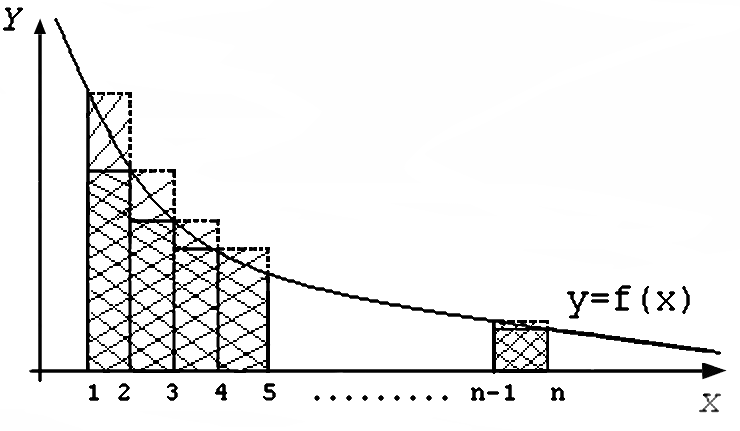
\includegraphics[width=6cm]{pics/Cauchy3}
    \end{figure}
\end{theorem}

\begin{lemma}
    Если $f>0$, $f \in [a, \upomega] \rightarrow [0, +\infty)$, $f\in R[a,b]$ $\forall b \in (a, \upomega)$
    \\
    Тогда $\int\limits_a^\upomega f$ - сх $\lra$ $F(x) = \int\limits_a^x f$, $\e M < \infty:  F(x) \leqslant M $ $\forall x \in [a, \upomega)$
\end{lemma}

\begin{proof}
    ($\Rightarrow$) очевидно
    \\
    ($\Leftarrow$) почти очевидно, $f \geqslant 0 \Rightarrow F \nearrow$ и огр $\Rightarrow \e \lim\limits_{x \rightarrow \upomega} F(x) = \int\limits_a^\upomega f < +\infty$
\end{proof}

\begin{proof}
    $f(n+1) \leqslant \int\limits_n^{n+1} f \leqslant f(n)$ (видно через суммы Дарбу) $|\sum\limits_{n=1}^N$
    \\
    $\sum\limits_{n=1}^N f(n+1) \leqslant \int\limits_1^{N+1} f \leqslant \sum\limits_{n=1}^N f(n)$, при $N \rightarrow +\infty$ получим наше уравнение
    \\
    1) Если $\sum\limits_1^\infty f (n)$ - сх $\lra$ $\sum\limits_1^N f(n) \leqslant A \in \R \Rightarrow F(N+1) = \int\limits_1^{N+1} f \leqslant A \in \R$ сх
    \\
    2) Если $\int\limits_1^\infty f$ - сх $\Rightarrow \sum\limits_1^N f(n+1) \leqslant \int\limits_1^{N+1} f \leqslant \int\limits_1^\infty f \in \R$ - огр $\Rightarrow \sum\limits_1^N f(n+1)$ сх
\end{proof}

\begin{examples}
    \begin{enumerate}
        \item $\sum\limits_{n=1}^\infty \frac{1}{n^2}$. Рассмотрим $\int\limits_1^\infty \frac{1}{x^2} = - \frac{1}{x} |_1^\infty = 0 - (-1)$ - сх
        \item $\sum\limits_{n=1}^\infty \frac{1}{n^\upalpha}$. Сх. при $\upalpha > 1$, расх. при $\upalpha \leqslant 1$ (аналогично интегралу $\int\limits_{1}^\infty \frac{1}{x^\upalpha}$)
    \end{enumerate}
\end{examples}

\newpage
\section{Признаки сравнения для несобственных интегралов.}

\begin{Theorem}[\RNumb{1} признак сравнения]
    \[f,g: [a, \upomega) \rightarrow \R,\q f,g \geqslant 0,\q f,g \in R[a,b],\q b \in (a, \upomega),\]
    \[0 \leqslant f(x) \leqslant g(x)\q \forall x \in [a, \upomega)\]
    Тогда $\int\limits_a^\infty g$ - сх $\Rightarrow$ $\int\limits_a^\upomega f$ - сх ($\int\limits_a^\upomega f$ - расх $\Rightarrow$ $\int\limits_a^\infty g$ - расх)
\end{Theorem}

\begin{Proof}
    \[F(b) := \int\limits_a^b f \leqslant \int\limits_a^b g \leqslant \int\limits_a^\upomega g \in \R\]
    То есть $\int\limits_a^\upomega f$ - сх, т.к. $F \nearrow$ и огр сверху на $[a, \upomega)$
\end{Proof}

\begin{Theorem}[\RNumb{2} признак сравнения]
    \[f, g: [a, \upomega) \rightarrow (0, +\infty)$, $f,g \in R[a,b]$ $\forall b \in (a, \upomega)\]
    Тогда если $\e \lim\limits_{x \rightarrow \upomega_-} \dfrac{f(x)}{g(x)} \in (0, +\infty)$, то $\int\limits_a^\upomega f$ и $\int\limits_a^\upomega g$ - сх или расх одновременно
\end{Theorem}

\begin{Proof}
    \[k:=\lim\limits_{x \rightarrow \upomega_-} \frac{f(x)}{g(x)} \in (0, +\infty)$, $\E := \dfrac{k}{2}\]
    \[\Rightarrow \e b \in (a, \upomega): \forall x \in (b, \upomega)\ |\frac{f(x)}{g(x)} - k| < \E \Rightarrow  \E < \frac{f(x)}{g(x)} <  3\E\]
    То есть с некоторого места $f(x) \leqslant g(x)$, а так как $\int\limits_a^\upomega = \int\limits_a^b + \int\limits_b^\upomega$ и $\int\limits_a^b f, \int\limits_a^b g$ - конечные числа, то $\int\limits_a^\upomega f$ и $\int\limits_a^\upomega g$ - сх или расх одновременно по первому признаку
\end{Proof}

\begin{Example}
    \[\int\limits_0^{+\infty} e^{-x^2} dx= \int\limits_0^1 + \int\limits_1^{+\infty}\]
    \begin{figure}[H]
        \centering
        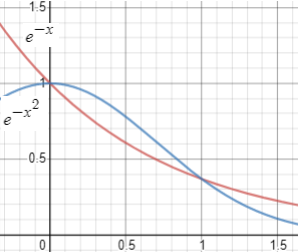
\includegraphics[width=4cm]{pics/ThirdGraph}
    \end{figure}
    \[e^{-x^2} \geqslant e^{-x} \Rightarrow x \in [0,1],\q \int\limits_0^1 e^{-x} = \frac{1}{e} \underset{\text{по \RNumb{1} пр. ср.}}{\Rightarrow} \int\limits_1^{+\infty} e^{-x^2}\text{ - сх}\]
\end{Example}

\begin{Example}
    \[\int\limits_1^{+\infty} \sin^2 \frac{1}{x} dx\]
    \[\lim\limits_{x\rightarrow\infty} \frac{\sin^2 \frac{1}{x}}{\frac{1}{x^2}} = 1 \in (0,+\infty) \Rightarrow \int\limits_1^{+\infty} \sin^2 \frac{1}{x} dx \text{ и } \int\limits_1^{+\infty} \frac{1}{x^2} dx \text{ - сх или расх одновр $\Rightarrow$ сх}\]
\end{Example}

\newpage
\section{Абсолютная и условная сходимость интегралов. Сходимость следует из абсолютной сходимости.}
\hypertarget{q27}{}

\begin{definition}
    $f: [a, \upomega) \rightarrow \R$, $f \in R[a,b]$ $\forall b \in (a, \upomega)$

    $\int\limits_a^\upomega f$ - сх абсолютно $\lra$ $\int\limits_a^\upomega |f|$ - сх

    $\int\limits_a^\upomega f$ - сх условно $\lra$ $\int\limits_a^\upomega f$ - сх, $\int\limits_a^\upomega |f|$ - расх
\end{definition}

\begin{utv}
    $\int\limits_a^\upomega f$ - сх абсолютно $\Rightarrow$ сходится
\end{utv}

\begin{proof}
    Пусть $\int\limits_a^\upomega |f|$ - сх $\lra$ (кр. Больцано-Коши) $\forall \E > 0$ $\e A \in (a, \upomega): \forall b_1, b_2 \in (A, \upomega)$ $|\int\limits_{b_1}^{b_2} |f|| < \E \Rightarrow $ т.к. $|\int\limits_{b_1}^{b_2} f| \leqslant |\int\limits_{b_1}^{b_2} |f|| < \E$, то по кр. Б-К $\int\limits_{b_1}^{b_2} f$ - сх
\end{proof}

\begin{Example}
    \[\int\limits_0^{+\infty} \cos (x^3) dx = \begin{vmatrix}
      x^3 = t\\
      x = \sqrt[3]{t}
    \end{vmatrix} = \frac{1}{3} \int\limits_0^\infty \cos t \frac{dt}{t^{\frac{2}{3}}} = \frac{1}{3} \frac{\sin t}{t^{\frac{2}{3}}}\Big|_0^\infty + \frac{2}{9} \int\limits_0^\infty \frac{\sin t}{t^{\frac{5}{3}}} = \frac{2}{9} \int\limits_0^\infty \frac{\sin t}{t^{\frac{5}{3}}}\]
    \[\text{Исследуем }\int\limits_0^\infty \frac{|\sin t|}{t^{\frac{5}{3}}} = \int\limits_0^1 \frac{|\sin t|}{t^{\frac{5}{3}}} + \int\limits_1^\infty \frac{|\sin t|}{t^{\frac{5}{3}}}:\]
    \[\text{a) }\int\limits_0^1 \frac{|\sin t|}{t^{\frac{5}{3}}}$, $|sin t| \leqslant t\text{ на }[0,1]\]
    \[\int\limits_0^1 \frac{t}{t^{\frac{5}{3}}} = \int\limits_0^1 t^{-\frac{2}{3}} = 3t^{\frac{1}{3}} |_0^1 = 3\text{ - сх} \underset{\text{по \RNumb{1} пр ср}}{\Rightarrow} \int\limits_0^1 \frac{|\sin t|}{t^{\frac{5}{3}}}\text{ - cх}\]
    \[\text{б) }\int\limits_1^\infty \frac{|\sin t|}{t^{\frac{5}{3}}},\q \frac{|\sin t|}{t^{\frac{5}{3}}} \leqslant \frac{1}{t^{\frac{5}{3}}}\]
    \[\int\limits_1^\infty \frac{1}{t^{\frac{5}{3}}} = -\frac{3}{2} t^{-\frac{2}{3}} |_1^\infty = \frac{3}{2}\text{ - сх} \underset{\text{по \RNumb{1} пр ср}}{\Rightarrow} \int\limits_1^\infty \frac{|\sin t|}{t^{\frac{5}{3}}}\text{ - cх}\]
    \[\text{Значит }\int\limits_0^\infty \frac{\sin t}{t^{\frac{5}{3}}}\text{ - абс сх }\Rightarrow \int\limits_0^{+\infty} \cos (x^3) \text{ - сх}\]
\end{Example}

\newpage
\section{Абсолютная и условная сходимость. Пример: $\int\limits_0^\infty \frac{\sin x}{x}$}

Определения и теорему см. в билете \hyperlink{q27}{27}
\begin{Example}
    \[\int\limits_0^\infty \frac{\sin x}{x} = \int\limits_0^{\frac{\pi}{2}} \frac{\sin x}{x} +  \int\limits_{\frac{\pi}{2}}^\infty \frac{\sin x}{x}\]
    \[1)\q \int\limits_{\frac{\pi}{2}}^\infty \frac{\sin x}{x} = \frac{-\cos x}{x} \Big|_\frac{\pi}{2}^\infty - \int\limits_\frac{\pi}{2}^\infty \frac{\cos x}{x^2} = \int\limits_\frac{\pi}{2}^\infty \frac{\cos x}{x^2}\]
    \[\text{Исследуем }\int\limits_\frac{\pi}{2}^\infty \frac{\cos x}{x^2}\text{ на абс сходимость}.\q \frac{|\cos x|}{x^2} \leqslant \frac{1}{x^2}, \text{ а} \int\limits_\frac{\pi}{2}^\infty \frac{1}{x^2}\text{ - сходится}\]
    \[\Rightarrow \text{ по 1 признаку сравнения } \int\limits_\frac{\pi}{2}^\infty \frac{|\cos x|}{x^2}\text{ - сх }\Rightarrow \int\limits_\frac{\pi}{2}^\infty \frac{\cos x}{x^2}\text{ - сх абс }\Rightarrow \int\limits_{\frac{\pi}{2}}^\infty \frac{\sin x}{x}\text{ - сх}\]
    \[2)\q \int\limits_0^{\frac{\pi}{2}} \frac{|\sin x|}{x}\]
    \[\text{Знаем, что }\lim\limits_{x \rightarrow 0} \frac{|\sin x|}{x} = 1.\text{ Кроме того, }\frac{|\sin x|}{x} < 1,\text{ значит на конечном}\]
    \[\text{промежутке }(0, \frac{\pi}{2}]\text{ интеграл конечный }\Rightarrow \int\limits_{0}^\infty \frac{\sin x}{x}\text{ - сх}\]
    \[\text{3) Покажем, что }\int\limits_{\frac{\pi}{2}}^\infty \frac{|\sin x|}{x}\text{ - расх. }\Rightarrow \int\limits_{0}^\infty \frac{|\sin x|}{x}\text{ - расх}\]
    \[|\sin x| \geqslant |\sin^2 x|,\q \int\limits_{\frac{\pi}{2}}^\infty \frac{\sin^2 x}{x} = \int\limits_{\frac{\pi}{2}}^\infty \frac{1 - \cos 2x}{x} = \frac{1}{2} \int\limits_{\frac{\pi}{2}}^\infty \frac{dx}{x}\text{(расх)} + \int\limits_{\frac{\pi}{2}}^\infty \frac{\cos 2x}{x}\text{(сх)}\]
\end{Example}

\newpage
\section{Признаки Дирихле и Абеля для несобственных интегралов (док-во одного из них).}

\begin{Theorem} [признак Абеля-Дирихле]
    \[f,g: [a, \upomega) \rightarrow \R,\q f \in C[a,\upomega),\q g \in C^1 [a,\upomega),\text{ g - монотонна.}\]
    Тогда если выполнено одно из условий:
    \[\text{(A) }\int_a^\upomega \text{f - сх, g - огр}\]
    \[\text{(Д) }F(x) := \int\limits_a^x \text{f - огр, }g(x) \underset{x \rightarrow \upomega_-}{\rightarrow} 0\]
    Тогда $\int\limits_a^\upomega f g$ - сх
\end{Theorem}

\begin{proof}
    (Д) без теоремы Бонне
    \[|F(x)| \leqslant C: g(x) \underset{x \rightarrow \upomega_-}{\rightarrow} 0\]
    \[\lim\limits_{b \rightarrow \upomega_-} \int\limits_a^b f g = \lim\limits_{b \rightarrow \upomega_-} (F g |_a^b - \int\limits_a^b F g') = F(a) g(a) - \lim\limits_{b \rightarrow \upomega_-} \int\limits_a^b F g'\]
    Исследуем интеграл на абс сходимость.
    \[\int\limits_a^b |F g'| \leqslant C \int\limits_a^b |g'| = \text{(т.к. g - монотонна)} C |\int\limits_a^b g'| = C |g(b) - g(a)| \underset{b \rightarrow \upomega_-}{\rightarrow} C |g(a)|\]
    Таким образом инт. ограничен $\Rightarrow$ изначальный сходится
\end{proof}

\newpage
\section{Признаки Дирихле и Абеля для рядов (док-во одного из них).}

\begin{definition}
    $A_n := \sum\limits_{k=1}^n a_k$, $A_0=0$
\end{definition}

\begin{Theorem} [преобразование Абеля]
    \[\sum\limits_{k=1}^n a_k b_k = A_n b_n + \sum\limits_{k=1}^{n-1} A_k (b_k - b_{k+1})\]
\end{Theorem}

\begin{Proof}
    \begin{multline*}
        $$\sum\limits_{k=1}^n a_k b_k = \sum\limits_{k=1}^n (A_k - A_{k-1}) b_k = \sum\limits_{k=1}^n A_k b_k - \sum\limits_{k=1}^n A_{k-1} b_k =\\
        =\sum\limits_{k=1}^n A_k b_k - \sum\limits_{k=0}^{n-1} A_k b_{k+1} = A_n b_n + \sum\limits_{k=0}^{n-1} A_k (b_k - b_{k+1})$$
    \end{multline*}
\end{Proof}

\begin{theorem} [признак Дирихле для рядов]
    Пусть $A_n$ - огр., $b_k \rightarrow 0$, $b_k$ - монотонно. Тогда $\sum\limits_{k=1}^\infty a_k b_k$ - сх
\end{theorem}

\begin{proof}
    \[\sum\limits_{k=1}^n a_k b_k = A_n b_n + \sum\limits_{k=1}^{n-1} A_k (b_k - b_{k+1}) \underset{n \rightarrow \infty}{\rightarrow} \sum\limits_{k=1}^{n-1} A_k (b_k - b_{k+1})\]
    Ряд $\sum\limits_{k=1}^\infty a_k b_k$ - сх $\lra$ $\sum\limits_{k=1}^\infty A_k (b_k - b_{k+1})$ - сх $\lra$ все частичные суммы огр
    \\
    $\sum\limits_{k=1}^N |A_k| |b_k - b_{k+1}| \leqslant M \sum\limits_{k=1}^N |b_k - b_{k+1}| = M |b_1 - b_{N+1}| \leqslant 2 M |b_1| \Rightarrow$ исх ряд сх
\end{proof}

\begin{theorem} [признак Абеля для рядов]
    Пусть $A_n$ - сх. $b_k$ - монотонно, $b_k$ - огр. Тогда $\sum\limits_{k=1}^\infty a_k b_k$ - сх
\end{theorem}

\newpage
\section{Применение интеграла Римана для вычисления площадей и объемов. Примеры.}

\begin{definition} [школьное]
    Пусть $P \in \R^2$("фигрура"), $\mathcal{P}$ - некоторый набор плоских "фигур$"$, $P_i \in \mathcal{P}$

    $g: \mathcal{P} \rightarrow [0, +\infty)$ - называется площадью, если:
    \begin{enumerate}
        \item $\forall P \in \mathcal{P}$, $S(P) \geqslant 0$
        \item $\forall P_1, P_2 \in \mathcal{P}: P_1 \cap P_2 = \o$ $\Rightarrow$ $S(P_1 \cup P_2)=S(P_1)+S(P_2)$
        \begin{definition}
            $\uptau: \R^2 \rightarrow \R^2$, сохраняет расстояние
        \end{definition}
        \item $\forall P \in \mathcal{P}$ $\uptau$-движения $S(\uptau(P))=S(P)$
    \end{enumerate}
\end{definition}

\begin{center}
    \textbf{Площадь криволинейной трапеции.}
\end{center}

\begin{figure}[H]
    \centering
    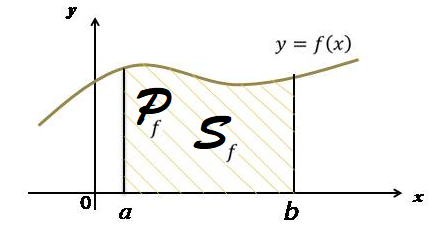
\includegraphics[width=6cm]{pics/Square}
\end{figure}

\begin{definition}
    Подграфиком $f \in R[a,b]$ называется $P_f := \{(x,y)| a \leqslant x \leqslant b,\ 0 \leqslant y \leqslant f(x) \}$
\end{definition}
\\
Возьмём разбиение и верх. и нижн. суммы Дарбу. $S$ - монотонна, т.е.

$$P_1 \subset P_2 \Rightarrow S(P_1) \leqslant S(P_2),\ S_*(\uptau)=S(P_*(\uptau)),\ S^*(\uptau)=S(P^*(\uptau))$$

$$P_*(f, \uptau) \subset P (f) \subset R^* (f, \uptau)$$

$$S(P_*(f, \uptau)) = S_*(f, \uptau) \rightarrow \int_a^b f,\ S(P^*(f, \uptau)) = S^*(f, \uptau) \rightarrow \int_a^b f,\ S(P_f) := \int_a^b f$$

\begin{example}
    Первая четверть эллипса с радиусами $(a,b)$.

    \[\frac{x^2}{a^2} + \frac{y^2}{b^2} = 1,\q y = b \sqrt{1 - \frac{x^2}{a^2}},\q S = \int\limits_0^a b \sqrt{1 - \frac{x^2}{a^2}} dx\text{ - сложно, перейдём в поляры}\]
    $\begin{cases}
       x = a \cos t\\
       y = b \sin t
     \end{cases}$
     \[\int\limits_0^a f(x) dx = \int\limits_{\frac{\pi}{2}}^0 b \sin t d(a \cos t) = a b \int\limits_{\frac{\pi}{2}}^0 \sin^2 t dt = -a b (t - \frac{\sin 2t}{2}) |_{\frac{\pi}{2}}^0 = 0 - (-\frac{\pi a b}{4}) = \frac{\pi a b}{4}\]
\end{example}

\newpage
\begin{center}
    \textbf{Вычисление объемов}
\end{center}

\begin{utv}
    Принцип Кавальери. Если у двух тел одни сечения на одном уровне, то их объемы равны.
\end{utv}

$\sum\limits_{k=0}^{n-1} S(\xi_k) \Delta_k$ - сумма Римана

$V= \int\limits_a^b S(x) dx$ - измельчаем плоскости

\begin{example}
    (на самом деле тела вращения можно считать как $V=\pi \int\limits_a^b f^2(x) dx$)
\end{example}

\newpage
\section{Путь. Длина пути. Спрямляемый путь. Аддитивность длины пути.}

\hypertarget{q32}{}

\begin{definition}
    $\upgamma: [a,b] \rightarrow \R^n,\q \upgamma = \begin{pmatrix}
      \upgamma_ 1\\
      \upgamma_2\\
      ...\\
      \upgamma_n
    \end{pmatrix},\q \upgamma_k: [a,b] \rightarrow \R$.
    Расстояние считается как $d(x,y)=||x - y||_2=\sqrt{\sum\limits_{k=1}^n (x_k-y_k)^2}$, $\upgamma$ - путь, если $\forall i \in \{1,...k\}\ \upgamma_i \in C[a,b]$
\end{definition}

\begin{definition}
    Путь называется $r$-гладким, если $\forall i \in \{1,...k\}\ \upgamma_i \in C^r[a,b]$
\end{definition}

\begin{definition}
    Два пути считаются эквивалентными если можно сделать замену переменной. Т.е. пусть $\upgamma: [a,b] \rightarrow \R$, $\w{\upgamma}: [\upalpha, \upbeta] \rightarrow \R$, тогда:
    \\
    $\upgamma \sim \w{\upgamma}$ $\lra$ $\e \upvarphi: [a,b] \rightarrow [\upalpha, \upbeta]$ - строго возрастающая, $\upalpha = \upvarphi (a)$, $\upbeta = \upvarphi (b)$, $\upgamma = \w{\upgamma} \circ \upvarphi$
\end{definition}

\begin{definition}
    Кривая - класс эквивалентности путей. $\forall$путь - представитель класса эквивалентности называется "параметризацией"
\end{definition}

\begin{Example}
    \begin{equation*}
    \upgamma_1: \begin{cases}
       x = \cos t & 0 \leqslant t \leqslant 2 \pi\\
       y = \sin t & 0 \leqslant t \leqslant 2 \pi
    \end{cases}\ \ \ \ \ \ \ \ \ \ \ \
    \upgamma_2: \begin{cases}
       x = \cos t^2 & 0 \leqslant t \leqslant 2 \pi\\
       y = \sin t^2 & 0 \leqslant t \leqslant 2 \pi
     \end{cases}
    \end{equation*}
    $\upgamma_1 \sim \upgamma_2$, определяют одну и ту же кривую (окружность)
\end{Example}

\begin{definition}
    Кривая называется $r$-гладкой, если у неё есть $r$-гладкая параметризация
\end{definition}

\begin{definition}
    $\upgamma$ - простой путь $\lra$ $\upgamma$ - биекция на $(a,b)$, т.е. $\forall t_1, t_2 \in (a,b): \upgamma(t_1) \neq \upgamma(t_2)$ (без самопересечений). \\
	Если $\upgamma(a) = \upgamma(b)$, $\upgamma$ - замкнутый путь.
\end{definition}

\begin{definition} [длины пути]
  	$\upgamma: [a,b] \rightarrow \R^m$, $\uptau - разбиение [a,b]: a=t_0<t_1<...<t_n=b$. Соединим $[\upgamma(t_k), \upgamma(t_{k+1})]$ отрезками - получим вписанную ломанную.
    $$\text{Длина $k$-ого звена: }\sqrt{\sum\limits_{j=0}^m (\upgamma_j(t_{k+1}) - \upgamma_j(t_k))^2}$$

    $$\text{Тогда длина вписанной ломанной: }l=\sum\limits_{k=0}^{n-1} \sqrt{\sum\limits_{j=0}^m (\upgamma_j(t_{k+1}) - \upgamma_j(t_k))^2}$$

    $$\text{Длиной пути назовём } S_\upgamma := \sup\limits_{\uptau} l_\uptau\text{ - всевозможных ломанных}$$
\end{definition}

\begin{definition}
    Путь называется спрямляемым, если $S_\upgamma < +\infty$
\end{definition}

\begin{utv}
    Аддитивность длины пути. $\upgamma: [a,b] \rightarrow \R$, $c \in (a,b)$, пусть $\upgamma_1$ - сужение $\upgamma$ на $[a,c]$, $\upgamma_2$ - сужение $\upgamma$ на $[c,b]$. Тогда $S_\upgamma = S_{\upgamma_1} + S_{\upgamma_2}$
\end{utv}

\begin{proof}
    а) $S_\upgamma \geqslant S_{\upgamma_1} + S_{\upgamma_2} ?$

    Пусть $\uptau_1$ - разбиение $[a,c]$, $\uptau_2$ - разбиение $[c,b]$,

    $\uptau = \uptau_1 + \uptau_2$, $l_{\uptau_1} + l_{\uptau_2} = l_\uptau \leqslant S_\upgamma$

    (т.к. $S_\upgamma - \sup$)

    Возьмём $\sup$ по всем разбиениям отрезка $[a,c]$

    $\Rightarrow$ $\sup\limits_{\uptau_1} (l_{\uptau_1} + l_{\uptau_2}) = S_{\upgamma_1} + l_{\uptau_2} \leqslant S_\upgamma$

    Теперь $\sup$ по всем разбиениям отрезка $[c,b]$

    $\Rightarrow$ $\sup\limits_{\uptau_1} (S_{\upgamma_1} + l_{\uptau_2}) = S_{\upgamma_1} + S_{\upgamma_2} \leqslant S_\upgamma$
    \\
    б) $S_\upgamma \leqslant S_{\upgamma_1} + S_{\upgamma_2} ?$

    Пусть $\uptau$ - разбиение $[a,b]$.

    Пусть $\uptau^* = \uptau \cup \{c\}$. $l_\uptau \leqslant l_{\uptau^*}$, $\uptau = \uptau_1 \cup \uptau_2$,

    где $\uptau_1$ - разбиение $[a,c]$, $\uptau_2$ - разбиение $[c,b]$.

    $l_\uptau \leqslant l_{\uptau^*} = l_{\uptau^1} + l_{\uptau^2} \leqslant S_{\upgamma_1} + S_{\upgamma_2}$

    Возьмём $\sup$ по всем разбиениям $\uptau$: $\sup\limits_{\uptau} (l_{\uptau}) = S_\upgamma \leqslant S_{\upgamma_1} + S_{\upgamma_2}$
\end{proof}

\begin{examples}
    Неспрямляемые пути:

    1) Кривая Пеано
    \begin{figure}[H]
        \centering
        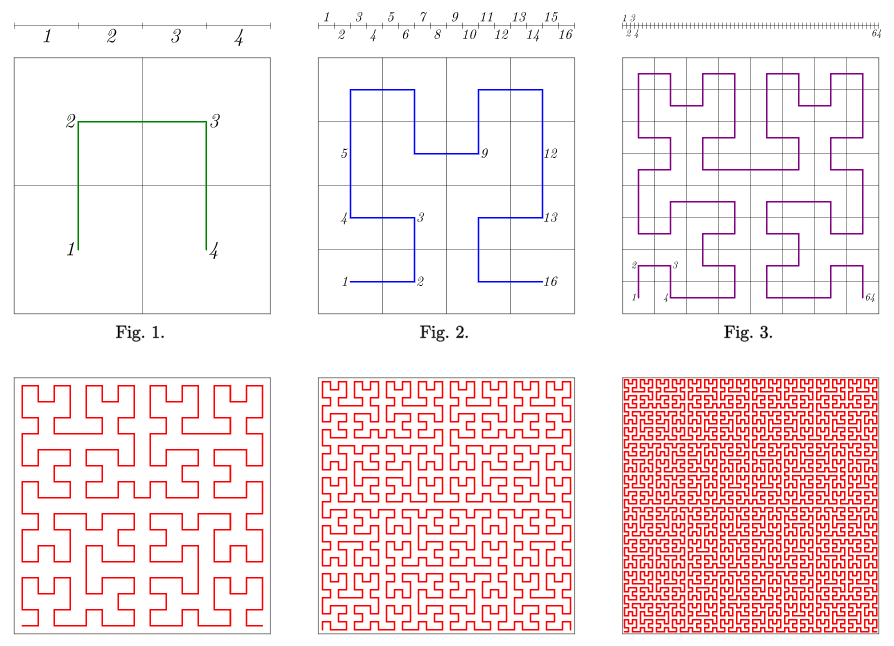
\includegraphics[width=9cm]{pics/Peano}
    \end{figure}

    В пределе $\upgamma: [0,1] \rightarrow [0,1]^2$ - сюръективное отображение. В итоге получается прямая заполняющая весь квадрат с пересеченями (в смысле дополнение до подкривых  пределе пусто)

    2) $y =
    \begin{cases}
       x \cos \frac{\pi}{x}, & x \neq 0\\
       0, & x = 0
     \end{cases}$

     \begin{figure}[H]
         \centering
         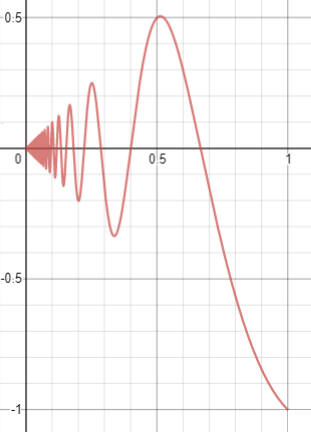
\includegraphics[width=3cm]{pics/cosfracpix}
     \end{figure}

    Докажем, что прямая не является спямляемой.
    \\
    Пусть $\uptau: 0 < \frac{1}{N} < \frac{1}{N -1} < ... < 1$, $t_N = \frac{1}{N}$, тогда
    \[y(t_k) = \frac{1}{k} \cos \pi k = \frac{1}{k} (-\pi)^k\]
    Длина $k$-ого звена:
    \[\frac{1}{k} - (-\frac{1}{k+1}) \geqslant \frac{2}{k} \Rightarrow l_\uptau \geqslant \sum\limits_{k=1}^N  \frac{1}{k}\Rightarrow \sup l_\uptau = +\infty\]
\end{examples}

\newpage
\section{Кривая. Длина кривой.}

Опр. см. в билете \hyperlink{q32}{32}
\begin{theorem} [о длинах эквивалентных путей]
    Пусть $\upgamma_1: [a_1,b_1] \rightarrow \R^m$, $\upgamma_2: [a_2,b_2] \rightarrow
    \R^m$. Если $\upgamma_1 \sim \upgamma_2$ $\Rightarrow$ $S_{\upgamma_1} = S_{\upgamma_2}$
\end{theorem}

\begin{proof}
    $\upgamma_1 \sim \upgamma_2$ $\Rightarrow$ $\e \upvarphi: [a_1, b_1] \rightarrow [a_2, b_2]$ - строго возрастающая, $\upgamma_1(t) = \upgamma_2(\upvarphi(t))$, $\upvarphi(\uptau_1) = \uptau_2$ - разбиение $[a_2,b_2]$,
    $$l_{\uptau_1} = \sum\limits_{k=0}^{n-1} \sqrt{\sum\limits_{j=0}^m (\upgamma_1(t_{k+1}) - \upgamma_1(t_k))^2} = l_{\uptau_2} \leqslant S_{\uptau_2}$$
    Перейдём к $\sup$ по всем $\uptau_1$: $\sup\limits_{\uptau_1} (l_{\uptau_1}) = S_{\uptau_1} \leqslant S_{\uptau_2}$

    Аналогично получим неравенство $S_{\uptau_2} \leqslant S_{\uptau_1}$
\end{proof}

\begin{remark}
    Корректность определения (с классами эквивалентности) длины пути следует из доказанной выше теоремы
\end{remark}

\newpage
\section{Теорема о вычислении длины гладкого пути.}

\begin{theorem}
    $\upgamma: [a,b] \rightarrow \R^m$ - $C^1$-гладкая кривая, тогда $\upgamma$ - спрямляется, $S_{\upgamma} = \int\limits_a^b |\upgamma'|$
\end{theorem}

\begin{proof}
    \\
    1) $\upgamma$ - спрямляемая?
    \\
    $\upgamma_j \in C^1[a,b]\ \forall j \in \{1,2,...,m\} \Rightarrow$(ф-ия достигает $\min$ и $\max$ на $[a,b]$ по т.Вейерштрасса)
    $$m_j \leqslant \upgamma_j \leqslant M_j,\ M := \sqrt{\sum\limits_{j=1}^m M_j},\ m := \sqrt{\sum\limits_{j=1}^m m_j},\ \upgamma' = \begin{pmatrix}
      \upgamma_1'\\
      \upgamma_2'\\
      ...\\
      \upgamma_n'
    \end{pmatrix}$$
    \\
    $\forall \uptau$-разбиения $[a,b]: l_\uptau = \sum\limits_{k=0}^{n-1} \sqrt{\sum\limits_{j=0}^m (\upgamma_1(t_{k+1}) - \upgamma_1(t_k))^2} = $
    \\
    (по т. Лагранжа $\forall k = 0,1,...n-1$ $\e \xi_k \in [t_k, t_{k+1}]: \upgamma_j(t_{k+1}) - \upgamma_j(t_k) = \upgamma_j'(\xi_k) \Delta_{t_k}$)
    \\
    $= \sum\limits_{k=0}^{n-1} \sqrt{\sum\limits_{j=0}^m (\upgamma_j'(\xi_k))^2 \Delta_{t_k}^2} = \sum\limits_{k=0}^{n-1} \sqrt{\sum\limits_{j=0}^m (\upgamma_j'(\xi_k))^2} \Delta_{t_k} \Rightarrow m \sum\limits_{k=0}^{n-1} \Delta_{t_k} \leqslant l_\uptau \leqslant M \sum\limits_{k=0}^{n-1}$
    \\
    $\Rightarrow m (b-a) \leqslant l_\uptau \leqslant M (b-a) \underset{sup}{\rightarrow} m (b-a) \leqslant S_\upgamma \leqslant M (b-a) \Rightarrow -\infty < S_\upgamma < +\infty$
    \\
    2) $S_{\upgamma} = \int\limits_a^b |\upgamma'|?$
    \\
    Пусть $\upgamma^{(k)}$ - сужение $\upgamma$ на $[t_k,t_{k+1}]$. Для него выполняется пункт (1):

    *переобозначим $\upgamma'$ как $\stackrel{\bullet}{\upgamma}$ из-за сложности обозначений*
    $$m_j^{(k)}=\min\limits_{t \in [t_k, t_{k+1}]} |\stackrel{\bullet}{\upgamma_j} (t)|,\ M_j^{(k)}=\max\limits_{t \in [t_k, t_{k+1}]} |\stackrel{\bullet}{\upgamma_j} (t)|$$
    $$m^{(k)} = \sqrt{\sum\limits_{j=1}^m (m_j^{(k)})^2},\ M^{(k)} = \sqrt{\sum\limits_{j=1}^m (M_j^{(k)})^2}$$
    $$m^{(k)} \Delta t_k \leqslant S_{\upgamma^{(k)}} \leqslant M^{(k)} \Delta t_k \Rightarrow \sum\limits_{k=1}^{n-1} \leqslant S_\upgamma \leqslant \sum\limits_{k=1}^{n-1} M^{(k)} \Delta t_k$$
    $$m_j^{(k)} \leqslant |\stackrel{\bullet}{\upgamma}_j^{(k)} (t) \leqslant M_j^{(k)}|\ t_k \leqslant t \leqslant t_{k+1},\ \forall j=1,...,m$$
    $$\text{Суммируем, возводим в квадрат, иззвлекаем корень:}$$
    $$m^{(k)} \leqslant |\stackrel{\bullet}{\upgamma}^{(k)} (t)| \leqslant M^{(k)}|\ t_k \leqslant t \leqslant t_{k+1}$$
    $$\text{Проинтегрируем по } \int\limits_{t_k}^{t_{k+1}} dt:\ m^{(k)} \Delta t_k \leqslant \int\limits_{t_k}^{t_{k+1}} |\stackrel{\bullet}{\upgamma}^{(k)} (t)| dt \leqslant M^{(k)} \Delta t_k$$
    $$\Rightarrow \sum\limits_{k=1}^{n-1} \leqslant \int\limits_{t_k}^{t_{k+1}} |\stackrel{\bullet}{\upgamma}^{(k)} (t)| dt \leqslant \sum\limits_{k=1}^{n-1} M^{(k)} \Delta t_k \text{, оценим } \sum\limits_{k=1}^{n-1} (M^{(k)} - m^{(k)} \Delta t_k):$$
    $$M^{(k)} - m^{(k)} = \frac{(M^{(k)})^2 - (m^{(k)})^2}{M^{(k)} + m^{(k)}} = \sum\limits_{j=1}^m (M_j^{(k)} - m_j^{(k)}) \frac{M_j^{(k)} + m_j^{(k)}}{M^{(k)} + m^{(k)}} \leqslant \sum\limits_{j=1}^m (M_j^{(k)} - m_j^{(k)})$$
    $$\upgamma_j \in C^1 [a,b] \Rightarrow \upgamma_j' \in C[a,b] \Rightarrow \text{р/н} \lra \forall \E > 0\ \e \updelta_j > 0:$$
    $$\uplambda(\uptau) < \updelta_j \Rightarrow 0 \leqslant M_j^{(k)} - m_j^{(k)} \leqslant \frac{\E}{m(b-a)} \underset{\updelta = \underset{1 \leqslant j \leqslant m}{\min \updelta_j}}{\stackrel{\sum\limits^m}{\Rightarrow}} 0 \leqslant M^{(k)} - m^{(k)} \leqslant \frac{\E}{b-a}$$
    $$\Rightarrow \sum\limits_{k=0}^{n-1} (M^{(k) - m^{(k)}} \Delta t_k < \frac{\E}{b-a} \sum\limits_{k=0}^{n-1} \Delta t_k = \E \Rightarrow S_\upgamma = \int\limits_a^b |\stackrel{\bullet}{\upgamma}|$$
\end{proof}

\newpage
\section{Функциональные последовательности и ряды. Поточечная и равномерная сходимость. Примеры.}

\begin{Definition}
    \[f_n : E \to \R \q E \subset \R\]
	\[\text{говорят, что функ. последовательность сходится поточечно}\]
	\[\text{к ф. } f : E \to \R \text{, если} \q \forall x \in E \q \forall \mathcal{E} > 0 \q \exists N_{(x, \mathcal{E})} : \q \forall n > N \]
	\[\abs{f_n(x) - f(x)} < \mathcal{E}\]
\end{Definition}

\begin{Definition}
    \[\text{Говорят, что функ. послед. сходится к } f \text{ равномерно на } E\]
	\[f_n \us{E}{\rightrightarrows} f \]
	\[\text{Если } \sup_{x \in  E} \abs{f_n(x) - f(x)} \us{n \to \infty}{\to 0}\]
	\[\rla \forall \mathcal{E} > 0 \q \exists N_{(\mathcal{E})} \q \forall n > N \q \sup_{x \in E} \abs{f_n(x) - f(x)} < \mathcal{E}\]
	\[\rla \forall \mathcal{E} > 0 \q \exists N_{(\mathcal{E})} \q \forall n > N \q \forall x \in E \q \abs{f_n(x) - f(x)} < \mathcal{E} \]
\end{Definition}

\begin{examples}
		\begin{enumerate}
			\item $\displaystyle  f_n(x) = \frac{sin^2(e^x) - \arctan(n^2 \sqrt{x})}{\sqrt{n}} \q\q x \in [0; +\infty)$
				\[0 \leq \sup_{[0, +\infty)} \abs{f_n(x)} \leq \frac{10}{\sqrt{n}} \to 0 \]
				\[\Ra f_n \us{[0, + \infty)}{\rightrightarrows} 0\]
			\item $f_n(x) = x^n - x^{2n} \q\q x \in [0, 1] $
				\[f_n(x) \us{n \to \infty}{\to } 0 \q \forall x \in [0, 1] \text{ - поточечно. Равномерно ли?}\]
				\[f'_n(x) = n x ^{n - 1} - 2nx^{2n-1} = x^{n - 1}(n - 2nx^n)\]
				\[x_n = \frac{1}{\sqrt[n]{2}} \text{ - крит. точка}\]
				\[f_n(x_n) = \frac{1}{2} - \frac{1}{4} = \frac{1}{4}\]
				\[\Ra \sup_{x \in [0, 1]} \abs{f_n(x)} = \frac{1}{4} \Ra \text{ равномерной сх-ти нет}\]
        \begin{figure}[H]
            \centering
    		    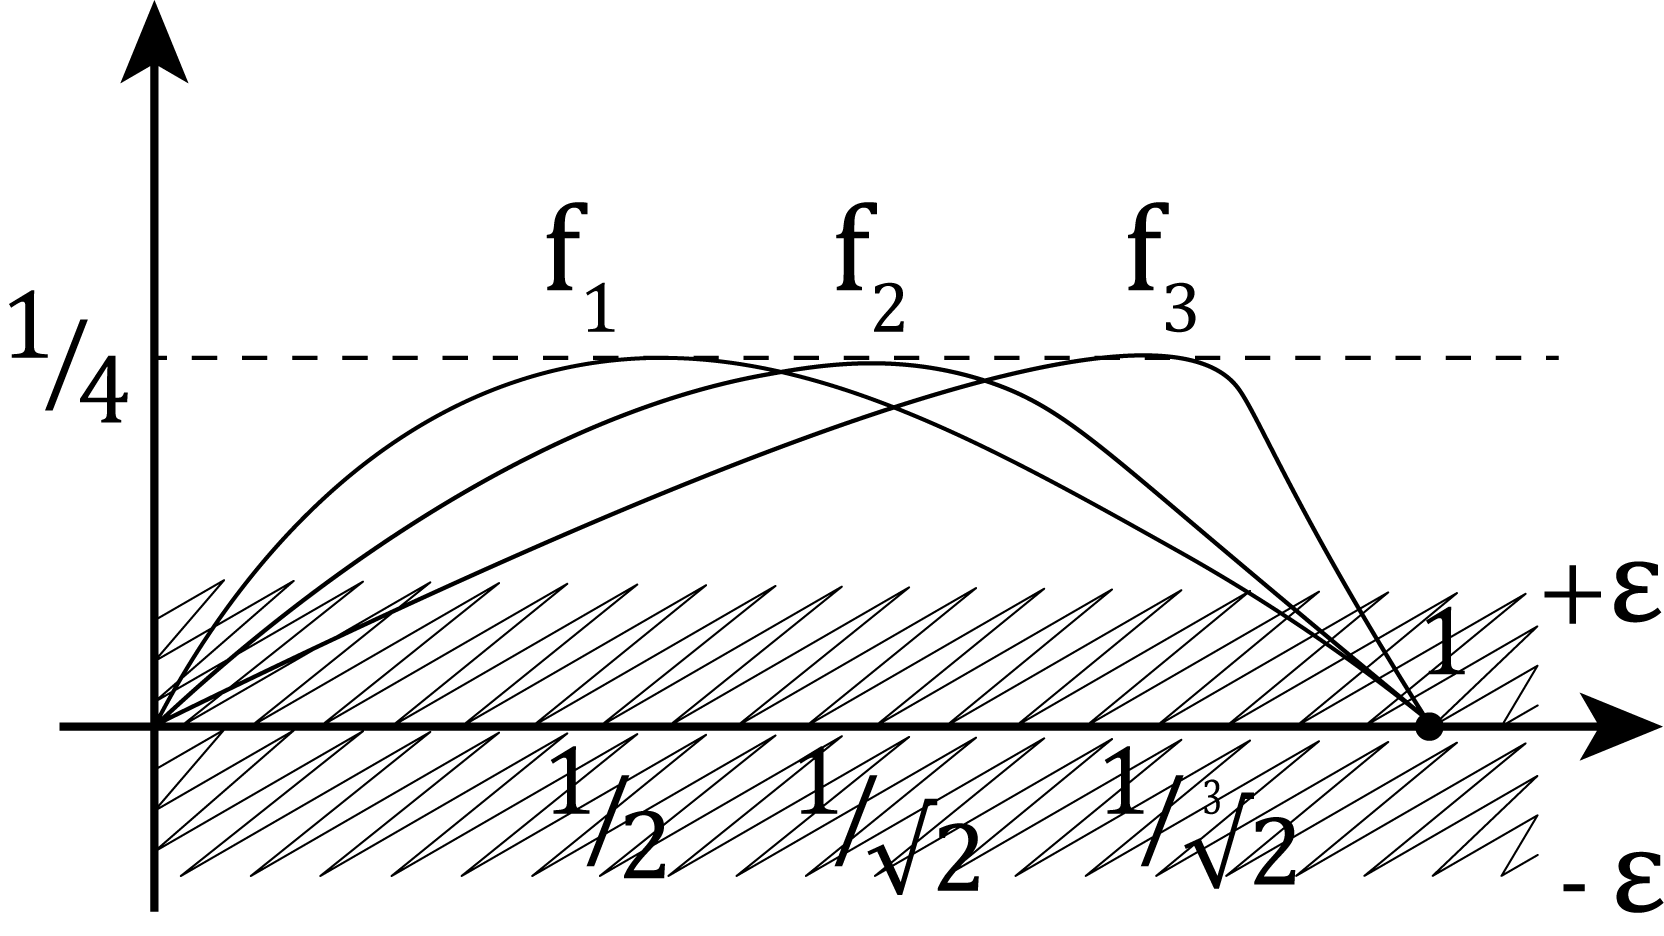
\includegraphics[width=6cm]{pics/f_n.png}
            \caption{Горбик убегает}
    		\end{figure}
		\end{enumerate}
\end{examples}

\begin{remark}
		Из равномерной сх-ти $\Ra$ поточечная
\end{remark}

\newpage
\section{Критерий Коши для равномерной сходимости функциональной последовательности.}

\begin{Theorem} [Критерий Коши для равномерной сходимости функ. послед.]
		\[f_n \us{E}{\rightrightarrows} f \rla \forall \mathcal{E} > 0 \q \exists N_\mathcal{E} :
		\forall m, n > N_\mathcal{E} \q\q \sup_{x \in E} \abs{f_n(x) - f_m(x)} < \mathcal{E} \]
\end{Theorem}

\begin{proof}
  ($\Ra$):
	\[f_n \rightrightarrows f \rla \sup \abs{f_n(x) - f(x)} \to 0\]
  \[\Ra \forall \mathcal{E} > 0 \q \exists N_\mathcal{E} > 0: \q \forall m, n > N_\mathcal{E} :\]
  \[\qq \sup \abs{f_n - f_m} \leq
      \sup(\abs{f_n - f} + \abs{f - f_m})
      < \frac{\mathcal{E}}{2} + \frac{\mathcal{E}}{2} = \mathcal{E}\]
  ($\La$):
	\[\forall x \in E \q \forall \mathcal{E} > 0 \q \exists N_\mathcal{E} :
	\forall m, n > N_{\mathcal{E}} \q \abs{f_n(x) - f_m(x)} < \mathcal{E}\]
	\[\text{т.е. } \{f_n(x)\} \text{ - сх. в себе } \rla \{f_n(x)\} \text{ имеет конеч. предел}\]
	\[f(x) = \lim_{n \to \infty} f_n(x) \text{ т.о. } f_n(x) \to f(x) \q \forall x \in E\]
  \[\qq \text{(т.е. f - поточеч. предел послед.)}\]
	\[\forall \mathcal{E} > 0 \q \exists N_\mathcal{E} : \forall m, n > N_\mathcal{E} \q \forall x \in E\]
	\[f_m(x) - \mathcal{E} < f_n(x) < f_m(x) + \mathcal{E} \us{n \to \infty}{\ra}
	  f_m(x) - \mathcal{E} \leq f(x) \leq f_m(x) + \mathcal{E}\]
	\[\Ra \abs{f_m(x) - f(x)} \leq \mathcal{E} < 2 \mathcal{E}\]
	\[\Ra \sup \abs{f_m(x) - f(x)} < \mathcal{E}\]
\end{proof}

\newpage
\section{Сохранение непрерывности при равномерном предельном переходе. Теорема Дини (б/д). Теорема о предельном переходе под знаком интеграла.}

\begin{Theorem} [о равномерном пределе непр. функции]
		\[f_n \text{ - непр в т. } x_0 \in E\]
		\[f_n \us{E}{\rightrightarrows} f\]
		\[\text{Тогда } f \text{ - непр. в т. } x_0\]
\end{Theorem}

\begin{Proof}
	\[\forall \mathcal{E} > 0 \q(\text{зафиксир.}) \]
	\[\text{Т.к. } f_n \rightrightarrows f \text{, то } \exists N_\mathcal{E} :
	\forall n > N_\mathcal{E} \q (\text{зафикс } n^* > N_\mathcal{E}) \q \sup_E \abs{f_n - f} < \frac{\mathcal{E}}{3}\q (*)\]
	\[\text{В частности, для } n^* > N_\mathcal{E} \q \sup_E \abs{f_n - f} < \frac{\mathcal{E}}{3}\]
	\[f_{n^*} \text{ - непр. в т } x_0 : \q \exists \delta > 0 \q \forall t \in E : \q
	\abs{t - x_0} < \delta \q \abs{f_{n^*}(t) - f_{n^*}(x_0)} < \frac{\mathcal{E}}{3}\]
	\[\text{Тогда } \forall x \in E : \q \abs{x - x_0} < \delta\]
	\[ \q \abs{f(x) - f(x_0)} \leq \abs{f(x) - f_{n^*}(x)} + \abs{f_{n^*}(x) - f_{n^*}(x_0)} + \abs{f_{n^*}(x_0) - f(x_0)} < \mathcal{E}\]
\end{Proof}

\begin{Consequence}
	\[\text{Если } f_n \in C(E), \q f_n \us{E}{\rightrightarrows} f \text{, то } f \in C(E)\]
\end{Consequence}

\begin{Theorem} [Дини]
	\[f_n \in C[a, b] \q\q f_n(x) \to f(x) \q(\text{поточ. на $[a, b]$})\]
	\[\text{причем}\q \forall x \in [a, b] \q f_n(x) \searrow \text{ (по n). \q т.е } f_{n+1}(x) \leq f_n(x) \]
	\[\text{Если } f \in C[a, b] \text{, то } f_n \us{[a, b]}{\rightrightarrows} f\]
\end{Theorem}

\begin{Theorem} [о предельном переходе под знаком интеграла]
	\[f_n \in R[a, b] \q f_n \us{[a, b]}{\rightrightarrows} f \in R[a, b]\]
	\[\text{Тогда } \int_a^b f_n \us{n \to \infty}{\to } \int_a^b f\]
\end{Theorem}

\begin{Proof}
		\[a < b\]
		\[\abs{\int_a^b f_n - \int_a^b f} \leq \int_a^b \abs{f_n - f} <
			\sup_{[a, b]} \abs{\us{\to 0}{f_n - f}} \cdot (b-a) \to 0\]
\end{Proof}

\begin{utv}
		Функ. ряд сход равномерно $\rla$ посл-ть частичных сумм сход равномерно
\end{utv}

\begin{Consequence}[1]
	\[f_n \in C[a, b] \q \sum_{n = 1}^N f_n \rightrightarrows f, \text{ тогда:}\]
	\[\begin{align}
		&\q1) \q f(x) = \sum_{n = 1}^\infty f_n \in C[a, b] \\
		&\q2) \q \int \sum_{n = 1}^\infty f_n = \sum_{n = 1}^\infty \int f_n
	\end{align}\]
\end{Consequence}

\begin{Consequence}[2]
	\[\text{Если } f_n(x) \geq 0 \q \forall  x \in [a, b] \q\q f_n \in C[a, b]\]
	\[\sum_{n = 1}^\infty f_n = f \in C[a, b] \]
	\[\text{То } \sum f_n \text{ - сход. равномерно на } [a, b]\]
\end{Consequence}
\newpage
\section{Дифференцируемость и равномерная сходимость.}

\begin{Theorem} [диф-сть и равном. сх-ть]
	\[f_n \in C^{1}[a, b] \q f_n' \us{[a, b]}{\rightrightarrows} g\]
	\[\text{и } \exists c \in [a,b] : \q \{f_n(c)\}^\infty_{n = 1} \text{ - сх} \]
	Тогда:
  \begin{enumerate}
    \item $f_n \rightrightarrows f \text{ на } [a, b]$
    \item $f \in  C^1[a, b] \text{ и } f' = g$
  \end{enumerate}
\end{Theorem}

\begin{Proof}
	\begin{multline*}
		(b) \q f_n(x) - f_n(c) = \int_c^x f'_n \us{n \to \infty}{\to } \int_c^x g = f(x) - f(c) \q\q
		f(c) = \lim_{n \to \infty} f_n (c) \\
		\text{ (по т. о 		предельном переходе под знаком интеграла)}
	\end{multline*}
	\[f(x) = \int_c^x g + f(c)\]
	\[\text{т.о } f_n(x) \to f(x) \text{ поточ. на }[a, b] \q\q f'(x) = g(x) \text{ непр
	(равн. предел непр ф.)}\]
	\[\Ra f \in C^1[a, b]\]
	\[(a) \q \text{ покажем, что } f_n \rightrightarrows f\]
	\[\sup_{x \in [a, b]} \abs{f_n(x) - f(x)} = \sup \abs{f_n(x) - f_n(c) + \underbracket{f_n(c) - f(c)}
	+ f(c) - f(x)} \leq \]
	\[\leq \sup \abs{\int_c^x f'_n - \int_c^x g + f_n(c) - f(c)} \leq
	\sup \abs{\int_c^x (f'_n - g)} + \abs{f_n(c) - f(c)} \q (*)\]
	\[f'_n \rightrightarrows g \Ra \abs{\int_c^x (f'_n - g)} \leq \underbracket{\sup \abs{ f'_n - g}}_{\to 0}
	\underbracket{(x-c)}_{\leq (a - b)} \]
	\[\forall  \mathcal{E} > 0 \q \exists N : \forall n > N \q \abs{\int_c^x (f_n' - g)} < \mathcal{E}\]
	\[\exists N_2 : \forall n > N_2 \q \abs{f_n(c) - f(c)} < \mathcal{E}\]
	\[\Ra (*) < 2\mathcal{E}\]
\end{Proof}

\begin{Example}
	\[f_n(x) = \frac{1}{n} \arctan(x^n)\]
	\[\sup_{\R} \abs{f_n(x)} \leq \frac{\pi}{2n} \to 0 \q \text{ т.е. } f_n \us{\R}{\rightrightarrows} 0 = f\]
	\[f'_n(1) = \frac{1}{n} \cdot \frac{1}{1 + x^{2n} } \cdot n \cdot x^{n - 1} \bigg|_1 = \frac{1}{2}\]
	\[\text{Но } (\lim_{n \to \infty}  f_n)'_{x = 1} = 0 \neq \lim_{n \to \infty} f_n'(1) \]
\end{Example}

\newpage
\section{Признак Вейерштрасса равномерной сходимости функциональных рядов.}

\begin{Theorem} [признак Вейерштрасса равн сх-ти]
		\[f_n : E \to \R\]
		\[\forall n \ \exists M_n \q \abs{f_n(x)} \leq M_n \q \forall x \in E\]
		\[\sum_{n = 1}^\infty M_n < \infty \text{ (сход. мажоранта)} \]
		\[\text{Тогда ряд } \sum_{n = 1}^\infty f_n(x) \text{ сх. равн. (и абс) на } E\]
\end{Theorem}

\begin{Proof}
	\[\forall \mathcal{E} > 0 \q \exists N: \forall m, n > N \q \abs{\sum_{k = m}^n M_k} < \mathcal{E}
	\rla \sum M_k < \infty\]
	\[\text{Тогда } \abs{S_n - S_{m - 1}} = \abs{\sum_{k = m}^n f_k(x)} \leq \sum_{k = m}^n \abs{f_k(x)} \leq
	\abs{\sum_{k = m}^n M_k } < \mathcal{E}\]
	\[\text{Т.е. } \abs{S_n - S_{m - 1} } < \mathcal{E} \text{ т.е. вып. кр. Коши для } S_n(x) =
	\sum_{k = 1}^n f_k(x) \]
	\[\text{част. суммы сх равн. } \Ra \text{ функ. ряд сх. равн.}\]
\end{Proof}
\newpage

\subfile{40.tex}

\newpage
\section{Замечания из конспектов, которые не вошли в билеты}
\subsection{Множества меры ноль}

\begin{definition}
    $E \subset \R$, говорят, что $E$ - мн-во меры ноль, если:

    $\forall \E > 0\ \underset{\underset{\text{набор откр. инт.}}{\text{не более чем сч.}}}{\e I_j = (\upalpha_j, \upbeta_j):} E \subset \underset{j \in \N}{\cup} I_j\ \sum\limits_{j=1}^\infty |I_j| < \E$ ($|I_j| = \upbeta_j - \upalpha_j$)
\end{definition}

\begin{examples}
    1) $\forall$ Конечное множество - мн-во меры ноль
    \[E = \{x_1, ..., x_n \}$, $I_j := (x_j - \dfrac{\E}{4n}, x_j + \dfrac{\E}{4n})$, $\sum\limits_{j=1}^n |I_j| = \dfrac{\E}{2}\]
    2) $A = \{a_j\}_{j \in \N}$ - счётное $\Rightarrow$ имеет меру 0.

    Как покрыть $\N$? $|I_j| = \dfrac{\E}{2^{j+1}}$ - геом. прогрессия
    \\
    3) Несчетное множество меры ноль:

    Канторовское мн-во (Канторовский компакт), построение:
    \[C = \us{n=1}{\os{\infty}{\cap}} C_n\]
    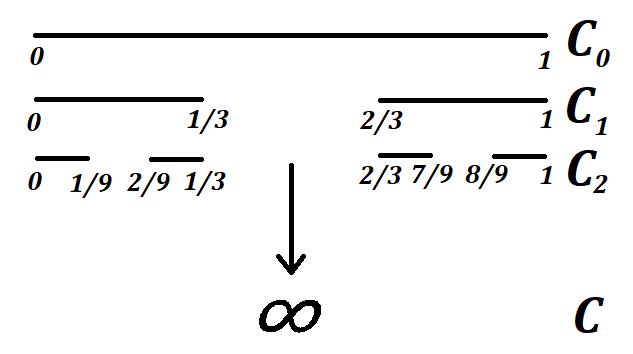
\includegraphics[scale=0.5]{Kantor}

    Определим $C_{\frac{1}{3^p}}$ как множество отрезков, получинных для $\E = \dfrac{1}{3^p}$ для крайних точек каждого отрезка из $C_p$ (они их покроют "вплотную" и по краям будет немного лишнего). На каждом шаге $p$ у нас $2^p$ отрезков
    \[\Rightarrow |C_{\frac{1}{3^p}}| = 5 \frac{2^{p-1}}{3^p} \underset{p \rightarrow \infty}{\rightarrow} 0\]
\end{examples}

\subsection{Критерий Лебега интегрируемости функции}

\begin{theorem}
    Пусть $f: [a,b] \rightarrow \R$, тогда:

    $f \in R[a,b]$ $\lra$ $f$ имеет ограниченное мн-во точек разрыва и меру 0
\end{theorem}

\begin{examples}
    1) Функция Дирихле $\mathcal{D}(x) =
    \begin{cases}
       1, & x \in \Q\\
       0, & x \notin \Q
     \end{cases}$

    $\mathcal{D} \notin R[0,1]$. Проверим по критерию Лебега. Множество точек разрыва - $\R$, но оно не множество меры 0 (слишком много точек).

    2) Функция Римана Ф$(x) =
    \begin{cases}
       0, & x \notin \Q\\
       \frac{1}{n}, & x = \frac{m}{n} \text{ - несократимая дробь}
     \end{cases}$
    \\
    Оказывается, она интегрируема по Риману на любом отрезке. Рассмотрим [0,1]:

    a) $\forall a \in \Q$ - точка разрыва Ф:

    Ф$(a) > 0$ по определению. С другой стороны как угодно близко найдётся иррациональная точка, в которой функция принимает значение 0.

    б) $\forall a \notin \Q$ - непрерывна:

    Для произвольного $\E > 0$ рассмотрим множество $M=\{ x \in \R: f(x) \ge \E \}$.

    Никакая иррациональная точка не лежит в $M$, поскольку в иррациональных точках функция $f$ обращается в ноль.

    Если $x\in M$, тогда $x$ есть рациональное число вида $x=\frac{m}{n}$, где $m\in\mathbb{Z},\ n\in\mathbb{N}$, дробь $\frac{m}{n}$ несократима, и тогда $f(x)=\frac{1}{n} \ge \E$ и, следовательно, $n \le \frac{1}{\E}$. Из ограничения на $n$ следует, что пересечение множества $M$ и любого ограниченного интервала состоит из конечного числа точек.

    Пусть $\upalpha$ - произвольное иррациональное число. По определению $f(\upalpha)=0$. Мы можем выбрать окрестность точки $\upalpha$ так, чтобы в ней не содержалась ни одна точка множества $M$. Если же $x \notin M$, то $f(x) < \E$. Таким образом, мы нашли интервал, который требуется в определении непрерывности.
\end{examples}
\end{document}
